% Created 2024-09-05 Thu 18:37
% Intended LaTeX compiler: pdflatex
\documentclass[aspectratio=169,xcolor={dvipsnames,svgnames}]{beamer}
\usepackage[utf8x]{inputenc}
\usepackage[T1]{fontenc}
\usepackage{graphicx}
\usepackage{longtable}
\usepackage{wrapfig}
\usepackage{rotating}
\usepackage[normalem]{ulem}
\usepackage{amsmath}
\usepackage{amssymb}
\usepackage{capt-of}
\usepackage{hyperref}
\usepackage{minted}
\usepackage{libertine}
\usepackage[normalem]{ulem}
\usepackage{varwidth}
\usepackage[Export]{adjustbox}
%\usepackage{enumitem}
\usepackage[linesnumbered,ruled,vlined]{algorithm2e}
\graphicspath{ {./careful-Isaac-Images/} {./org-download-images/} }
\usepackage[date=year,%
backend=biber,%
style=alphabetic,%
maxnames=5,%
minnames=3,%
maxalphanames=4,%
minalphanames=3,%
backref=true,%
doi=false,%
isbn=false,%
url=false,%
eprint=false]{biblatex}
\DefineBibliographyStrings{english}{%
backrefpage  = {\lowercase{s}ee p.}, % for single page number
backrefpages = {\lowercase{s}ee pp.} % for multiple page numbers
}
\addbibresource{/home/bvraghav/bibliography.bib}
%% Math typesetting
%% --------------------------------
\usepackage{amsmath}
\usepackage{amssymb}
\usepackage{amsfonts}
\usepackage{bbold}
% Operators with limit-style sub and superscript
\DeclareMathOperator*{\E}{\mathbb{E}}
\hypersetup{%
colorlinks=true,%
allcolors=magenta,%
%linkbordercolor = {white},%
%<your other options...>,
}
\usetheme{boxes}
\usecolortheme{crane}
\usefonttheme{serif}
\useinnertheme{rectangles}
\useoutertheme{}
\date{}
\title{mca101 : computer graphics}
\subtitle{2d geometry representation}
\author{%
%\noindent{} \\[2em]
\normalsize Raghav B. Venkataramaiyer
}
\institute{%
CSED TIET Patiala India.
}
\date{\scriptsize \today}
\setbeamercolor{alerted text}{fg=red!80!black}
%% Setup outline at begin section
%% -------------------------------------------------------
\AtBeginSection[]               % Section
{
\begin{frame}{outline}
\tableofcontents[currentsection,hideallsubsections]
\end{frame}
}
\AtBeginSubsection[]            % SubSection
{
\begin{frame}{outline}
\tableofcontents[currentsection,currentsubsection,subsectionstyle=show/shaded/hide]
\end{frame}
}
\setbeamerfont{structure}{shape=\scshape,family=\sffamily}
\setbeamertemplate{section page}
{
\begin{centering}
\begin{beamercolorbox}[sep=12pt,center]{part title}
\usebeamerfont{section title}\insertsection\par
\end{beamercolorbox}
\end{centering}
}

\setbeamercovered{transparent}
\makeatletter
\newcommand{\RemoveAlgoNumber}{\renewcommand{\fnum@algocf}{\AlCapSty{\AlCapFnt\algorithmcfname}}}
\newcommand{\RevertAlgoNumber}{\algocf@resetfnum}
\makeatother
\SetKwProg{Fn}{Function}{ is}{end}
\SetKwBlock{Cont}{}{end}
\hypersetup{
 pdfauthor={B.V. Raghav},
 pdftitle={mca101 : computer graphics},
 pdfkeywords={},
 pdfsubject={},
 pdfcreator={Emacs 29.4 (Org mode 9.6.24)}, 
 pdflang={English}}
\begin{document}

\maketitle

\section{2d geometry --- introduction}
\label{sec:orgaa5f78e}

\subsection{Straight Lines}
\label{sec:org9fbbb1a}

\begin{frame}[label={sec:org5d59ee3}]{\(y = mx + c\)}
\begin{align}
  \notag
  y = f(x) &= mx + c
\end{align}

\begin{center}
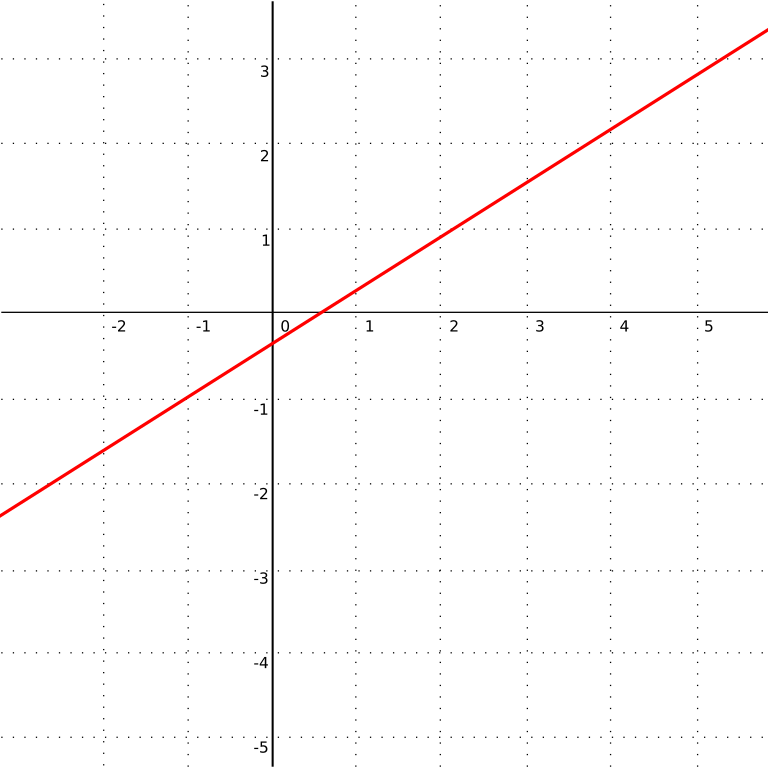
\includegraphics[width=0.3\linewidth]{images/st-line.png}
\end{center}
\end{frame}

\begin{frame}[label={sec:orgf417977}]{parametric form}
\begin{columns}
\begin{column}{.5\columnwidth}
For any two vectors \(\mathbf{u},\mathbf{v}\in V\), a
point on the line segment joining them is given
parameterised by \(t\in[0,1]\), as

\begin{align}
  \notag
  \mathbf{p} = f(t) &= (1-t)\mathbf{u} + t\mathbf{v}
\end{align}
\end{column}
\end{columns}
\end{frame}

\begin{frame}[label={sec:org54c3e00}]{parametric form}
\begin{columns}
\begin{column}{.5\columnwidth}
Any point on a line in the direction of unit vector
\(\mathbf{u}:\|\mathbf{u}\|_2^2=1\), and an incident
point \(\mathbf{p}_0\) may be given parameterised by
\(t\in\mathbb{R}\) as,

\begin{align}
  \notag
  \mathbf{p} = f(t) &= \mathbf{p}_0 + t\mathbf{u}
\end{align}
\end{column}
\end{columns}
\end{frame}

\begin{frame}[label={sec:org9f98420}]{hesse normal form}
\begin{columns}
\begin{column}{.5\columnwidth}
\begin{center}
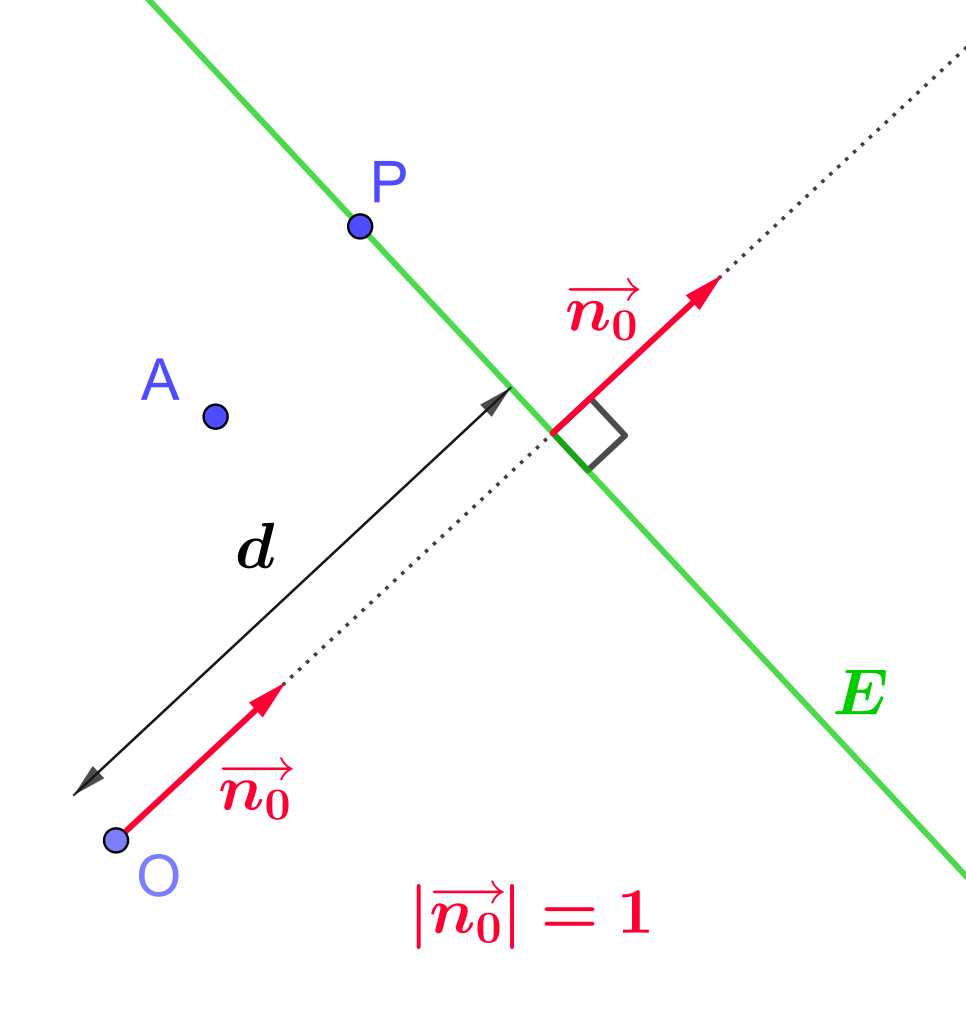
\includegraphics[width=0.7\linewidth]{images/Hesse_normalenform.svg.png}
\end{center}

Distance from the origin \(O\) to the line \(E\) calculated
with the Hesse normal form. Normal vector in red, line
in green, point O shown in blue.
\end{column}

\begin{column}{.6\columnwidth}
Given, \\[0pt]
Normal to the line
\(\mathbf{n}_0:\|\mathbf{n}_0\|_2^2=1\), and \\[0pt]
its distance from origin, \(d\);

\vspace{\baselineskip}
The point on the line is given implicitly as the locus
of all points \(\mathbf{p}\) that satisfy,

\begin{align}
  \notag
  \mathbf{n}_0 \cdot \mathbf{p} - d &= 0
\end{align}
\end{column}
\end{columns}
\end{frame}

\subsection{Conics}
\label{sec:org508473c}


\begin{frame}[label={sec:orgaf002e5}]{circle}
\begin{columns}
\begin{column}{.4\columnwidth}
\begin{figure}[htbp]
\centering
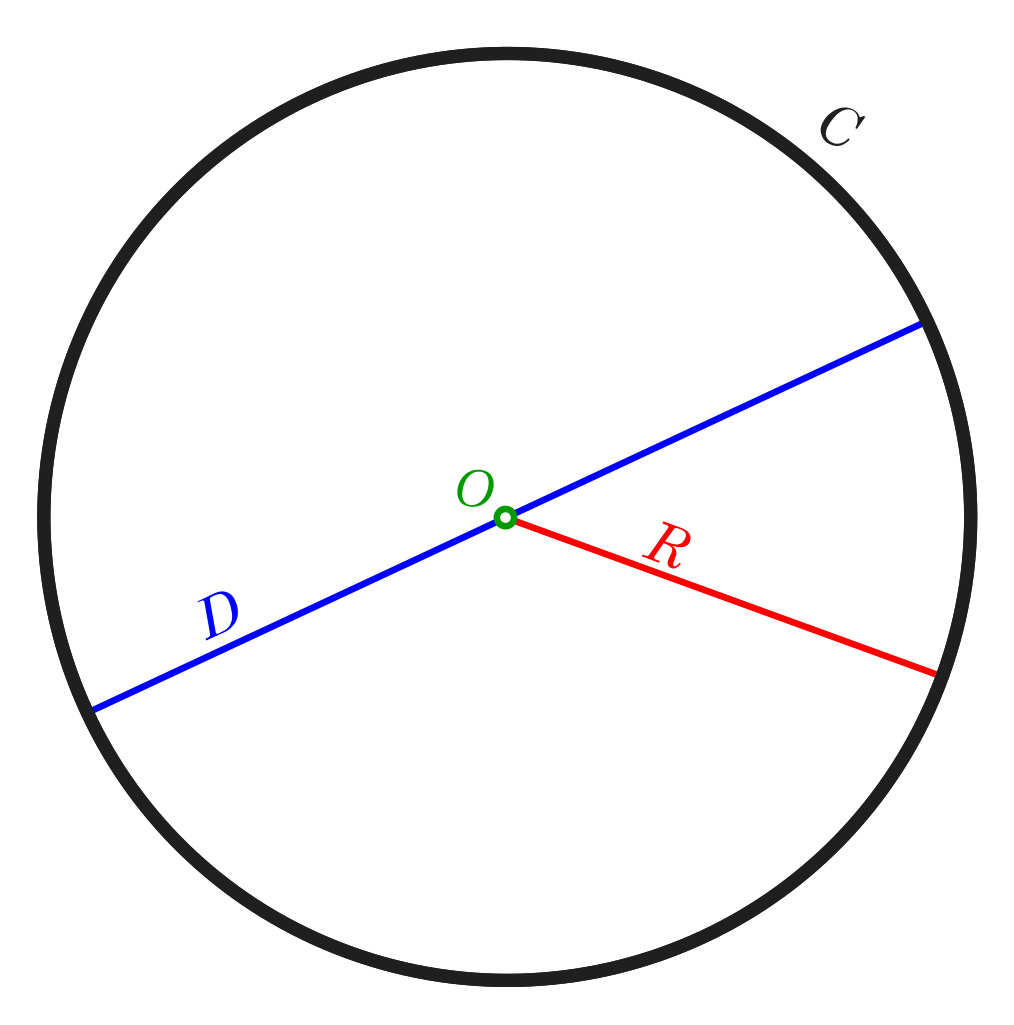
\includegraphics[width=.9\linewidth]{images/Circle-withsegments.svg.png}
\caption{Image Courtesy: \href{https://en.wikipedia.org/wiki/File:Circle-withsegments.svg}{Wikipedia}}
\end{figure}
\end{column}

\begin{column}{.6\columnwidth}
Implicit Form:
\begin{align}
  \notag
  f\left(\begin{matrix}x\\y\end{matrix}\right)
  &= x^2 + y^2 - r^2 = 0
\end{align}

Parametric Form:
\begin{align}
  \notag
  f(r,t)
  &= \begin{bmatrix}r\cos t\\r\sin t\end{bmatrix}
\end{align}
\end{column}
\end{columns}
\end{frame}
\begin{frame}[label={sec:org89f1ee1}]{ellipse}
\begin{columns}
\begin{column}{.4\columnwidth}
\begin{figure}[htbp]
\centering
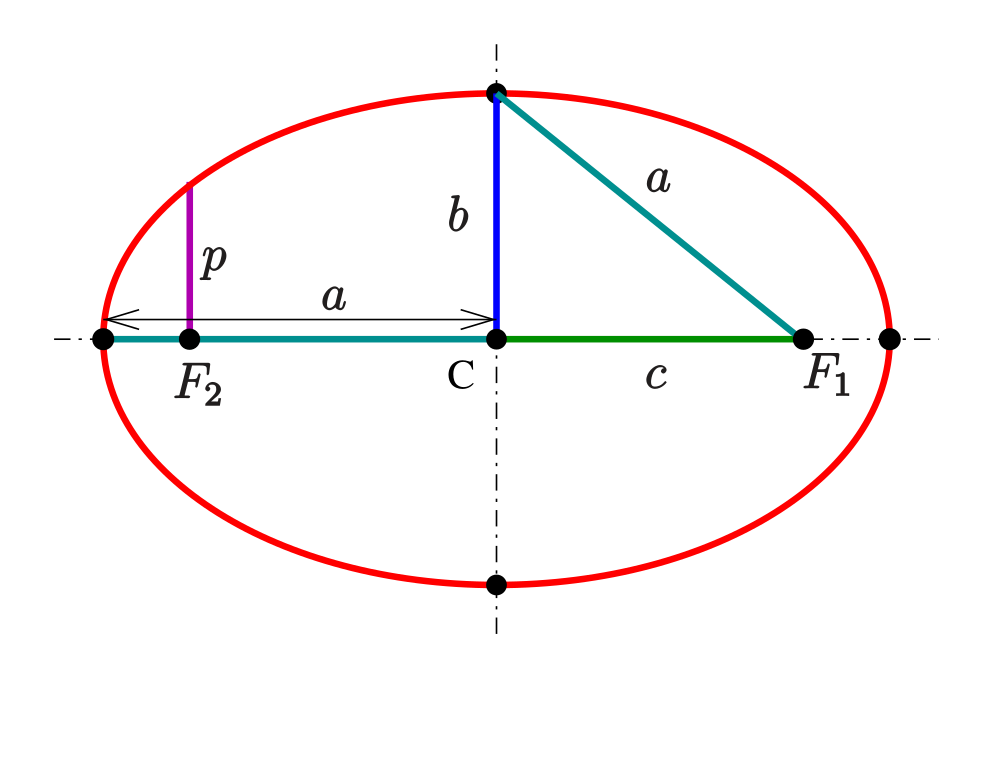
\includegraphics[width=.9\linewidth]{images/Ellipse-param.svg.png}
\caption{Image Courtesy: \href{https://commons.wikimedia.org/wiki/File:Ellipse-param.svg}{Wikipedia}}
\end{figure}
\end{column}

\begin{column}{.6\columnwidth}
Standard form
\begin{align}
  \notag
  f\left( \begin{matrix}x\\y\end{matrix} \right)
  &= \frac{x^2}{a^2} + \frac{y^2}{b^2} - 1 = 0
\end{align}

Parametric Form
\begin{align}
  \notag
  f(t;a,b) &= \begin{bmatrix}
    a\cos t \\ b \sin t
  \end{bmatrix}
\end{align}
\end{column}
\end{columns}
\end{frame}


\section{mid-point algorithm}
\label{sec:orge5f46b1}

\subsection{Fundamentals}
\label{sec:org718eff1}

\begin{frame}[label={sec:org1936f4e}]{problem}
\begin{columns}
\begin{column}{.5\columnwidth}
In a quantised (pixelated or discrete) 2d plane, find
the set of points that visually approximate a given
curve, say a straight line or a conic.
\end{column}
\end{columns}
\end{frame}

\begin{frame}[label={sec:org1c33f5c}]{method}
\begin{columns}
\begin{column}{.5\columnwidth}
Iteratively, increment along one axes, \\[0pt]
with respect to which, the slope of the curve is
gentle.

{\vspace{\baselineskip}}
Decide whether it is required to increment along the
perpendicular axis or not.

{\vspace{\baselineskip}}
Increment if required.
\end{column}
\end{columns}
\end{frame}

\begin{frame}[label={sec:org2e97cf0}]{example}
\begin{center}
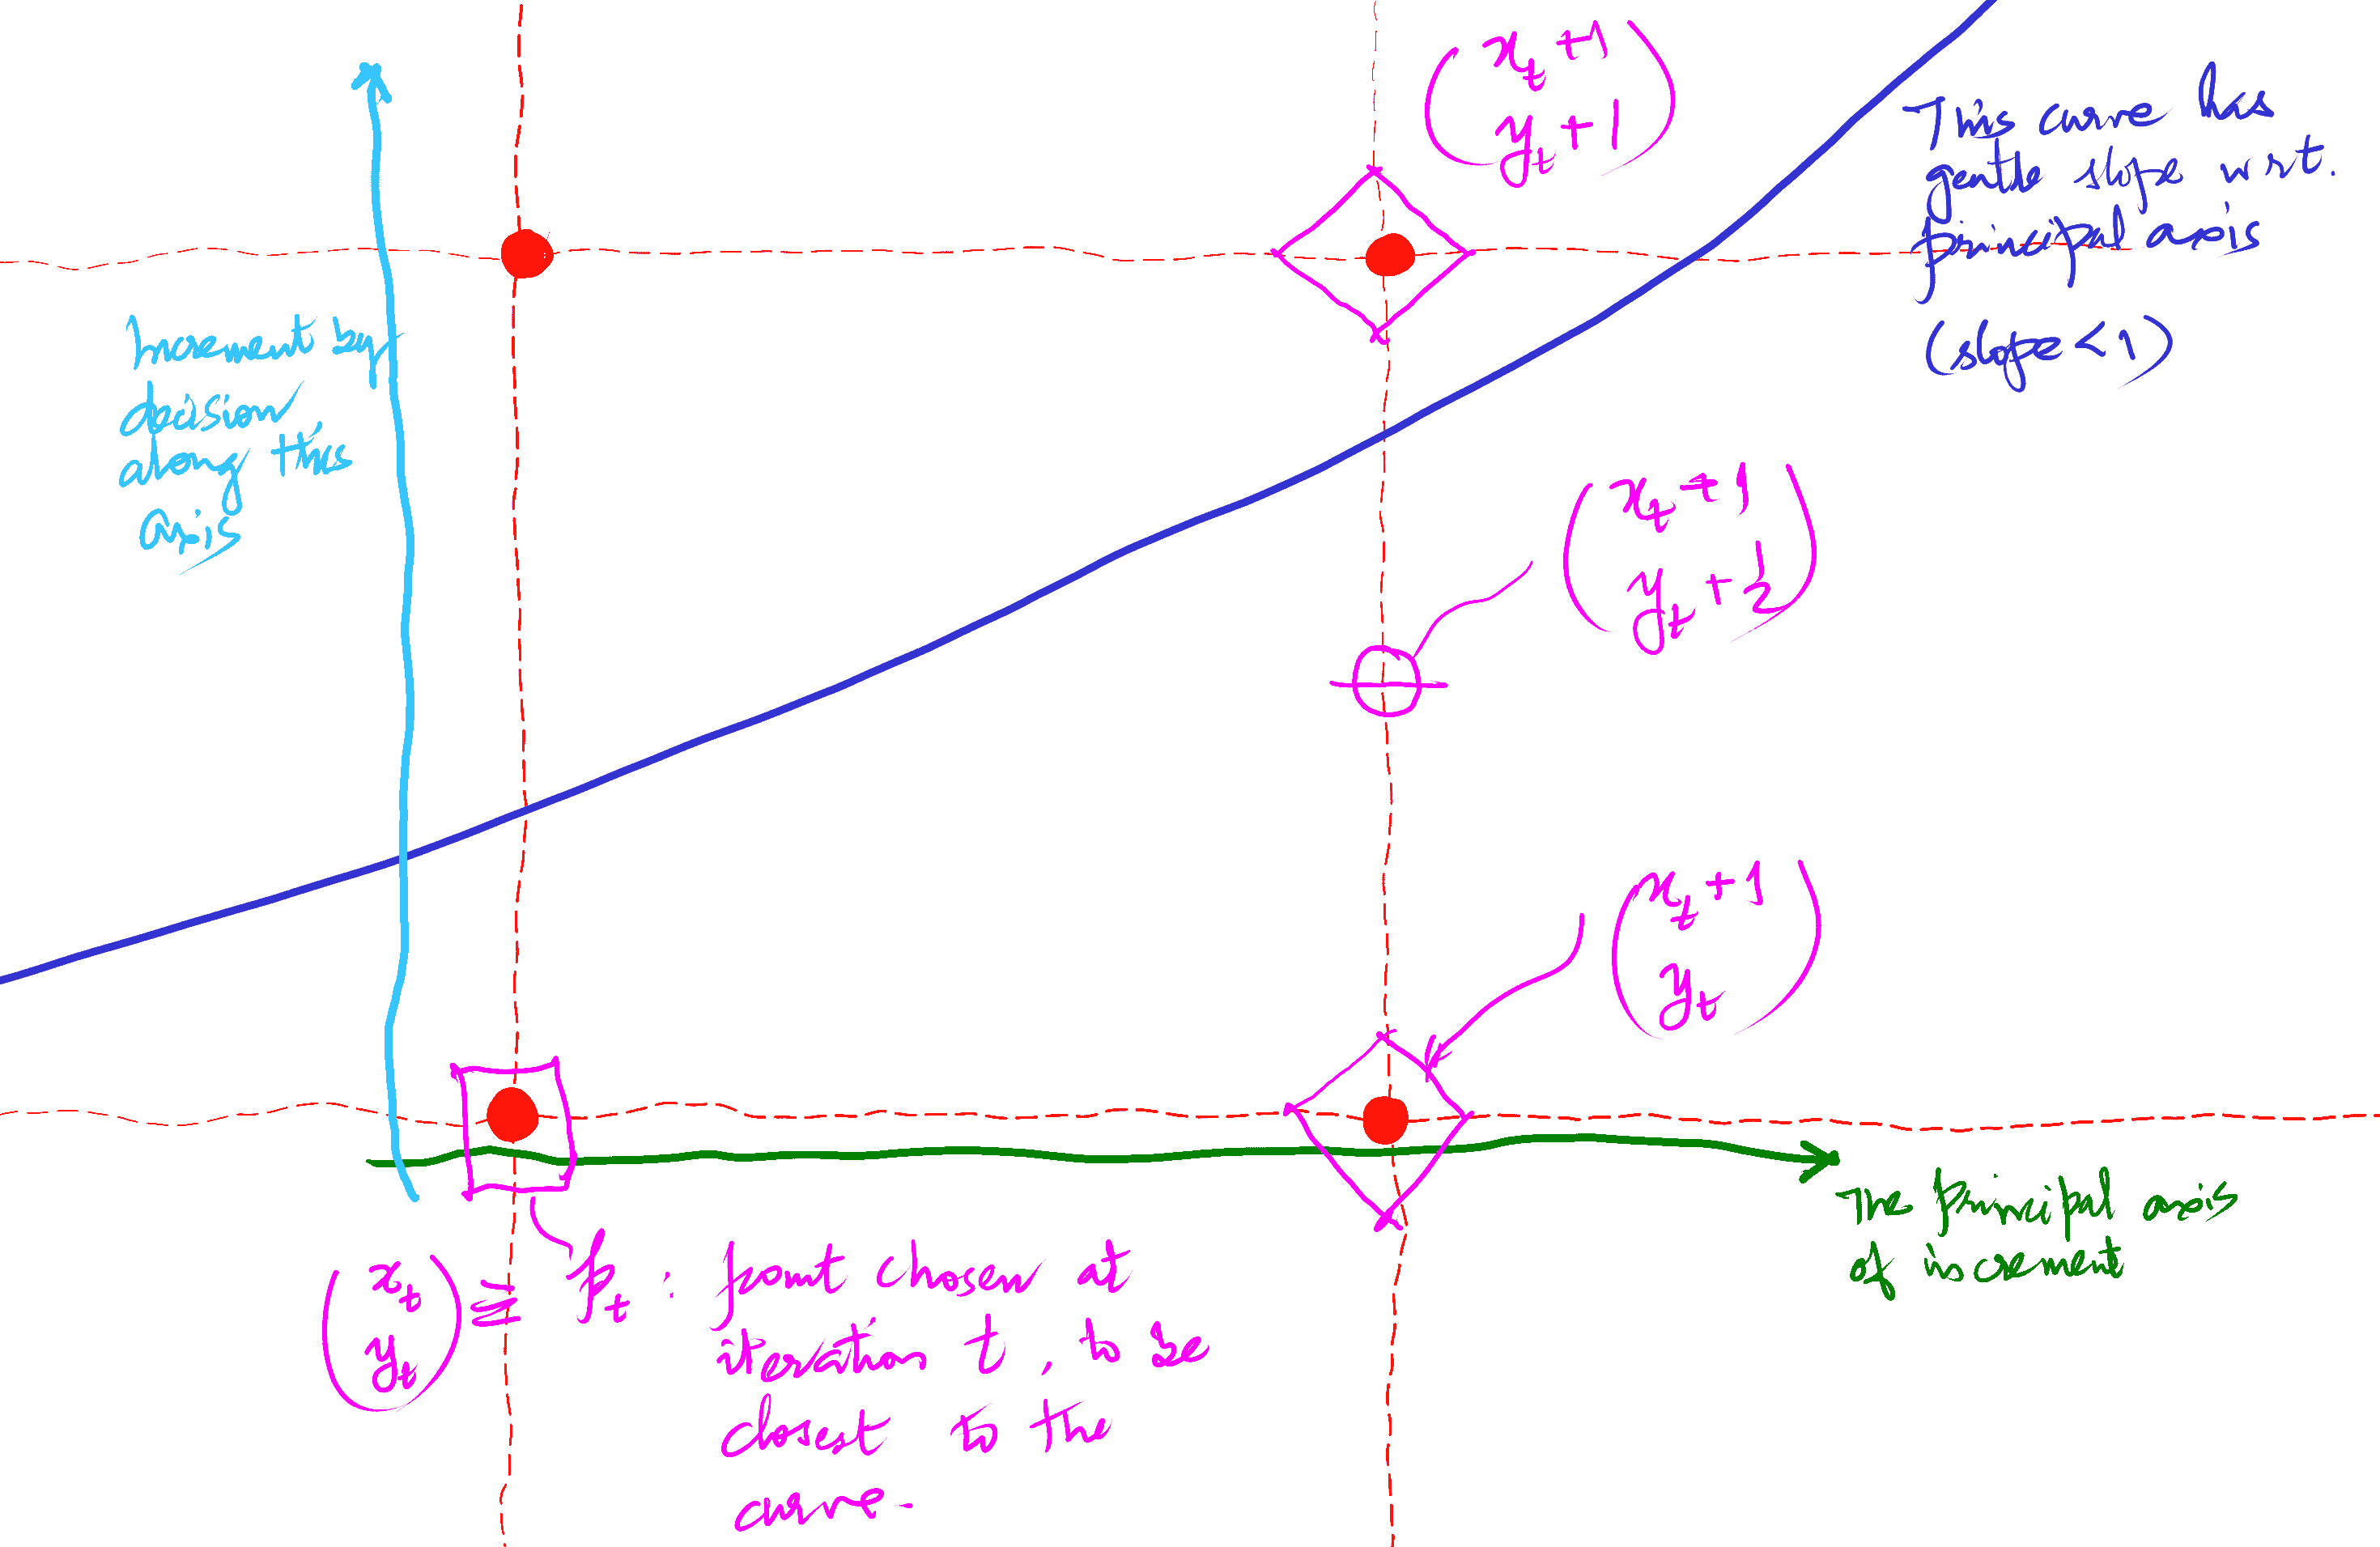
\includegraphics[width=0.8\linewidth]{images/basic-midpoint-algo.png}
\end{center}
\end{frame}

\begin{frame}[label={sec:org6bc102b}]{example}
\begin{center}
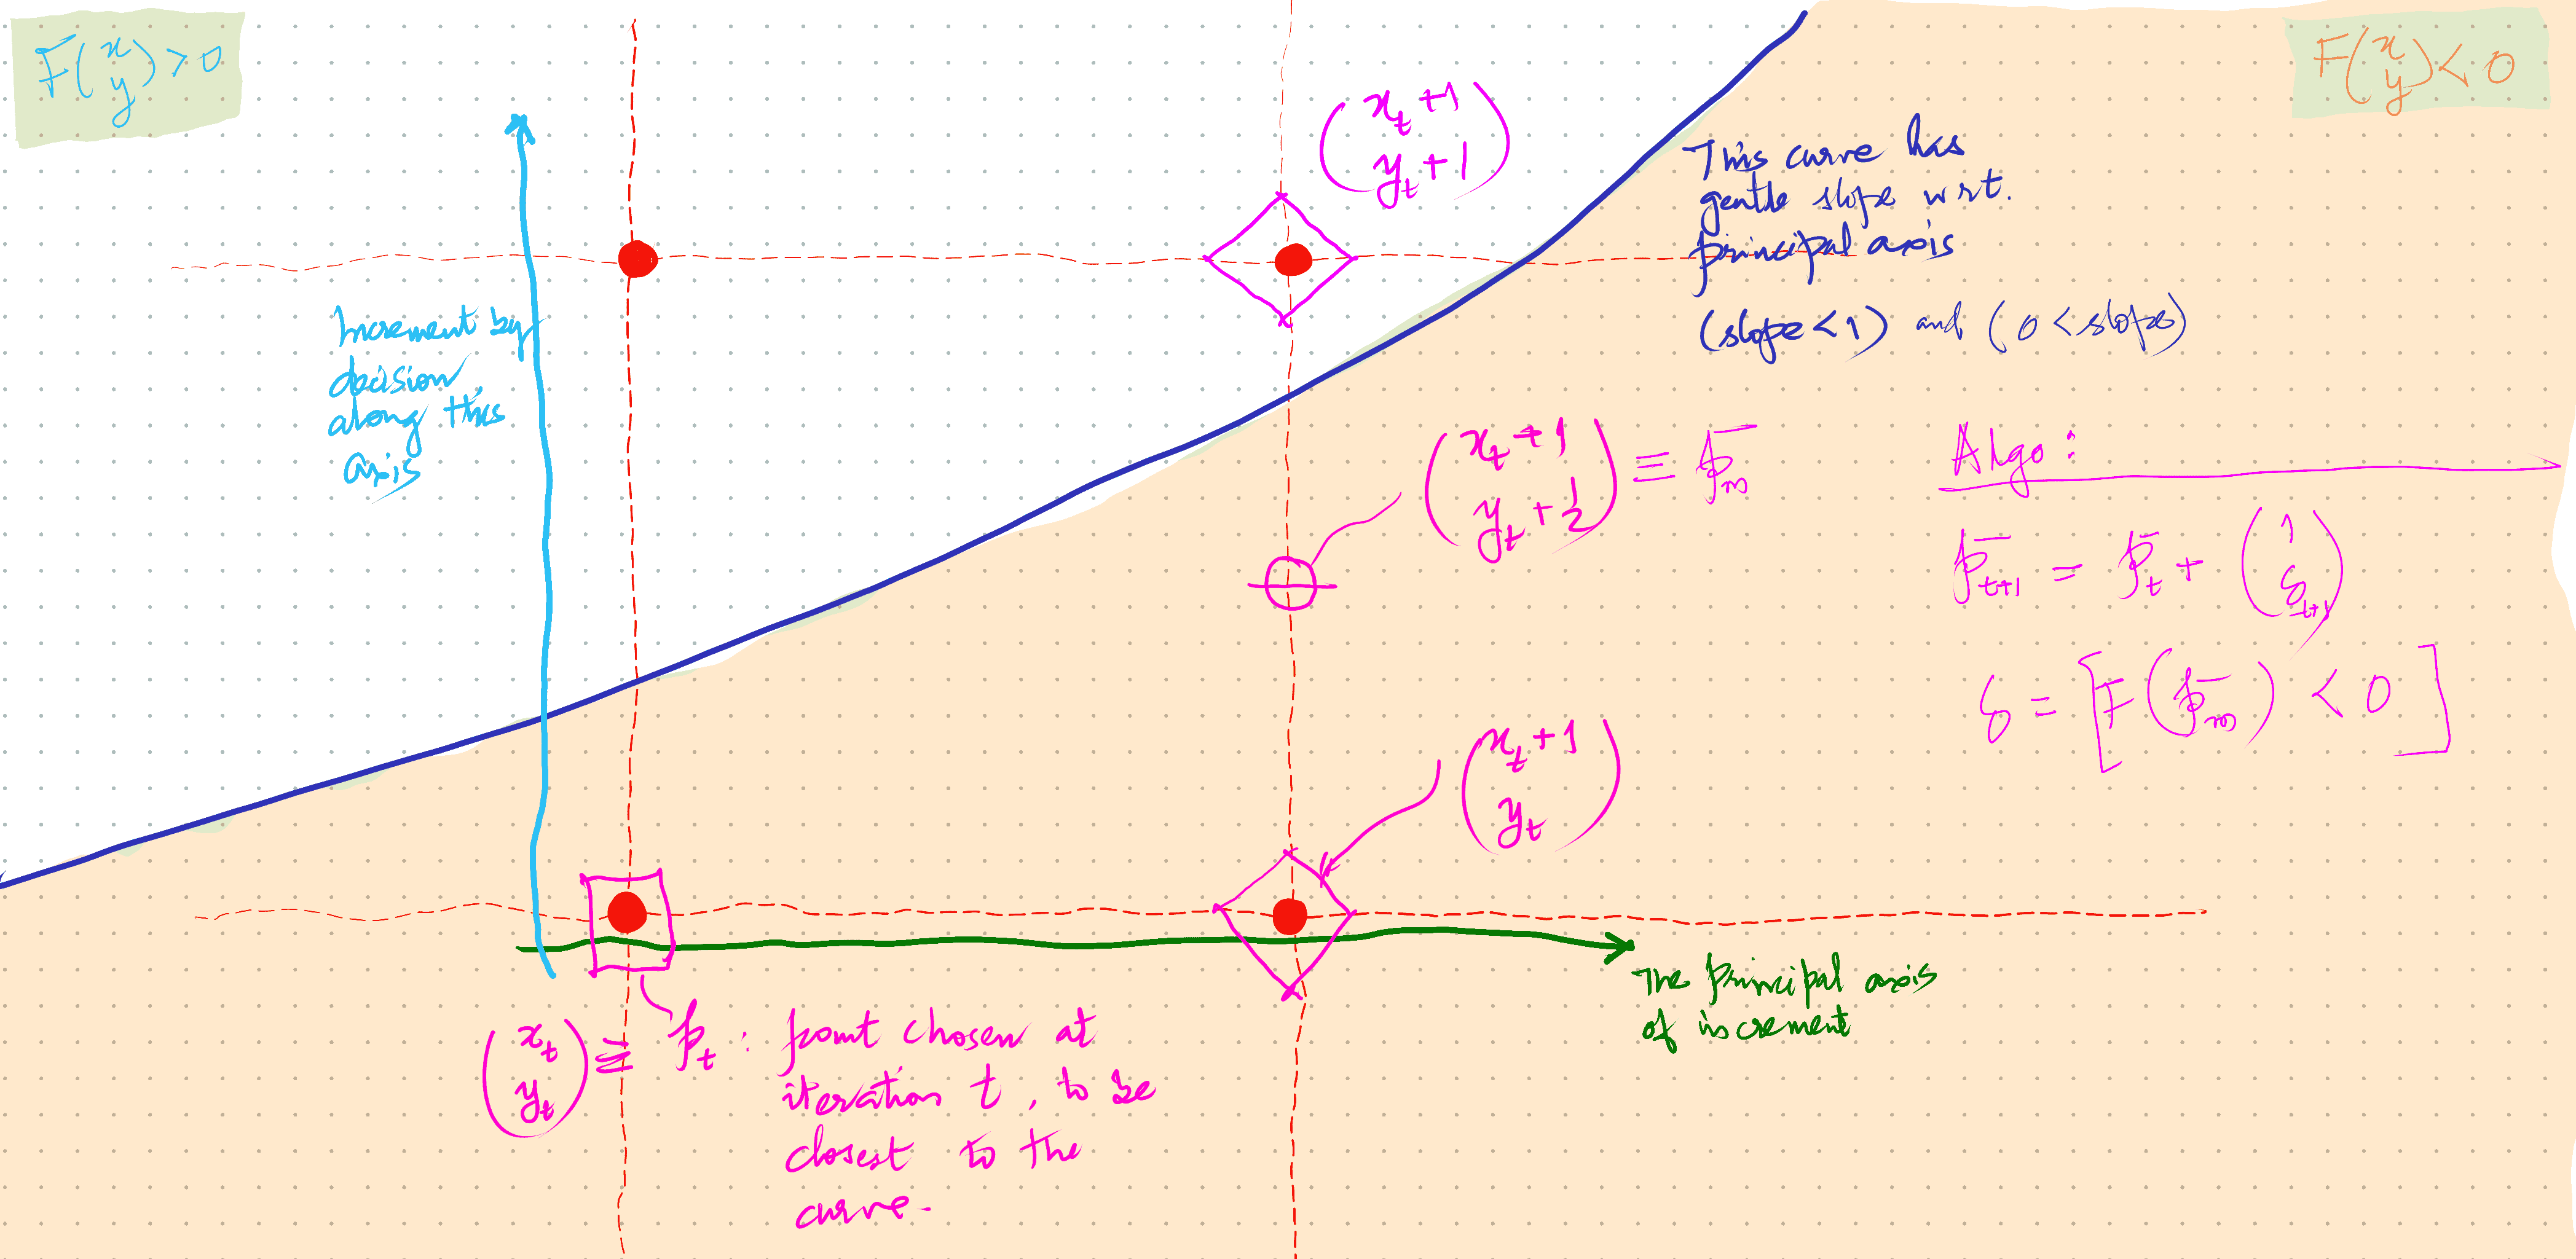
\includegraphics[width=\linewidth]{images/0--mid-point-algo_annotated.png}
\end{center}
\end{frame}

\begin{frame}[label={sec:orge40821a}]{conditions for application of mid-point algorithm}
\begin{columns}
\begin{column}{.45\columnwidth}
Mid-point algorithm is applicable to a curve within a
given finite interval, \alert{iff}

\begin{enumerate}
\item The curve increases monotonically;
\item The curve increases gradually.
\end{enumerate}


In other words,
\begin{align}
  \notag
  0 &\leqslant \mathrm{d}y \leqslant \mathrm{d}x
\end{align}
\end{column}
\end{columns}
\end{frame}

\begin{frame}[label={sec:orgcb7baa7}]{generic algo}
\begin{algorithm}[H]
  \caption{Generic Mid-point Algorithm}
  \DontPrintSemicolon
  \KwIn{$x_0,x_{\mathrm{max}}\in\mathbb{Z}$\hfill\scriptsize
    Start and end x-coordinates.}

  \KwIn{$F:\mathbb{R}^2\to\mathbb{R}$ \hfill
    \scriptsize Signed Distance Function from the curve.}

  \KwOut{$C \equiv
    \{\mathbf{p}_0,\ldots,\mathbf{p}_{\mathrm{max}} \}
    \subset \mathbb{Z}^2$ \hfill \scriptsize Curve in
    discrete 2D space.}

  {$\mathbf{p}_0 \gets \begin{bmatrix} x_0 \\ \lceil
    y_0\rceil \end{bmatrix} \vdash F\left(\begin{matrix}
      x_0 \\ y_0 \end{matrix}\right) = 0$}


\For{$t\in\{1,\ldots,\mathrm{max}\}$}{
  $\mathbf{p}_{\mathrm{mid}}\gets\mathbf{p}_{t-1}+\begin{pmatrix}1\\
    \frac12\end{pmatrix}$

  $\delta_t\gets I[F(\mathbf{p}_{\mathrm{mid}})<0]$

  $\mathbf{p}_{t}\gets\mathbf{p}_{t-1}+\begin{pmatrix}
    1 \\ \delta_{t} \end{pmatrix}$
  }
\end{algorithm}
\end{frame}


\subsection{Straight Line}
\label{sec:org06a9bdf}

\begin{frame}[label={sec:orgd164dca}]{characterising straight lines}
\begin{align*}
  F(x,y)
  &= Ax-By+C \\
  0 \leqslant \mathrm{d}y / \mathrm{d}x \leqslant 1 \quad
  &\mapsto \quad 0 \leqslant A \leqslant B
  &&\textsc{\ldots case 1} \\
  -1 \leqslant \mathrm{d}y / \mathrm{d}x \leqslant 0 \quad
  &\mapsto \quad 0 \leqslant A \leqslant -B
  &&\textsc{\ldots case 2} \\
  0 \leqslant \mathrm{d}x / \mathrm{d}y \leqslant 1 \quad
  &\mapsto \quad 0 \leqslant B \leqslant A
  &&\textsc{\ldots case 3} \\
  -1 \leqslant \mathrm{d}x / \mathrm{d}y \leqslant 0 \quad
  &\mapsto \quad 0 \leqslant -B \leqslant A
  &&\textsc{\ldots case 4}
\end{align*}

\href{https://tiet-mca101.github.io/lectures/images/2024-09-02-Note-08-32\_annotated.pdf}{Read more [\ldots{}]​}
\end{frame}

\begin{frame}[label={sec:orgc549294}]{mid-point algo for st. line}
Case 1. \(\alert{0<A<B}\)

\begin{algorithm}[H]
  \caption{Mid-Point Algorithm for Straight Line}
  \DontPrintSemicolon

  \Fn(\hfill {\scriptsize Base case.}){\upshape
    \textsc{mid-point-algo-st-line-base}\,
    ($x_1, y_1, N, a, b, c$)}{
    \KwIn{$x_1, y_1, N \in \mathbb{Z} \vdash 0<N$
      \hfill \scriptsize Start coordinates and num
      points.}

    \KwIn{$a,b,c\in\mathbb{Z} \vdash 0\leqslant a < b;
      b\;\mathrm{even}$ \hfill \scriptsize
      Coefficients: $F(x,y)=ax\alert{-by}+c$.}

    \KwOut{$C \equiv
      \{(x_1,y_1),\ldots,(x_N,y_N)
      \} \subset \mathbb{Z}^2$ \\\scriptsize An ordered
      sequence; a curve in discrete 2D space.}
    
    $\delta_1\gets ax_1\alert{-by_1- \frac b2} +c$
    \hfill{\scriptsize $\frac b2\in\mathbb{Z}$ because
      $b$ even.}

    \For{$t\in\{2,\ldots,N\}$}{
      $x_t\gets x_{t-1} + 1$

      $\delta_t\gets \delta_{t-1} + a - b\cdot
      I[0\leqslant\delta_{t-1}]$

      $y_t \gets y_{t-1} + I[0\leqslant\delta_t]$
    }

    \Return{$C \equiv \{(x_1,y_1), \ldots,
      (x_N, y_N) \}$ }

  }
\end{algorithm}
\end{frame}

\begin{frame}[label={sec:org92bb87e}]{mid-point algo for st. line}
Case 1. \(\alert{0<A<B}\)

\begin{algorithm}[H]
  \caption{Mid-Point Algorithm for Straight Line
    (alternate) \hfill {\scriptsize\textsc{[\ldots
        contd]}}}
  \DontPrintSemicolon
  \KwIn{$x_1, y_1, N\in\mathbb{Z} \vdash 0<N$
    \hfill \scriptsize Start and end x-coordinates.}

  \KwIn{$a,b,c\in\mathbb{Z} \vdash 0\leqslant a < b;
    b\;\mathrm{even}$ \hfill \scriptsize Coefficients:
    $F(x,y)=ax\alert{-by}+c$.}

  \KwOut{$C \equiv
    \{(x_1,y_1),\ldots,(x_N,y_N)
    \} \subset \mathbb{Z}^2$ \\\scriptsize An ordered
    sequence; a curve in discrete 2D space.}

  \textbf{Init:} $C\gets\emptyset$ \hfill {\scriptsize
    Initialise as array.}

  \textbf{Init:} $(x,y,\delta) \gets (x_1, y_1, 0)$
  \hfill {\scriptsize Initialise as integers.}
  
  $\delta\gets ax\alert{-by- \frac b2} +c$
  \hfill{\scriptsize $\frac b2\in\mathbb{Z}$ because
    $b$ even.}

  $C\cdot\textsc{push}\left((x,y)\right)$ \hfill
  {\scriptsize $(x,y)$ is a tuple.}
\end{algorithm}
\end{frame}

\begin{frame}[label={sec:orgc0923d4}]{mid-point algo for st. line}
Case 1. \(\alert{0<A<B}\)

\begin{algorithm}[H]
  \RemoveAlgoNumber
  \setcounter{AlgoLine}{6}
  \caption{{\scriptsize\textsc{[contd \ldots]}}
    Mid-Point Algorithm for Straight Line (alternate)}

  \For{$t\in\{2,\ldots,N\}$}{

    $x\gets x + 1$ \hfill {\scriptsize Increment along
      x-axis.}

    $\delta\gets \delta + a - b\cdot I[0\leqslant\delta]$
    \hfill {\scriptsize Update decision param
      $\delta$.}

    $y \gets y + I[0\leqslant\delta]$ \hfill {\scriptsize
      Update along y-axis based on decision param.}

    $C\cdot\textsc{push}\left((x,y)\right)$ \hfill
    {\scriptsize $(x,y)$ is a tuple.}

  }

  \Return $C$
\end{algorithm}
\end{frame}

\begin{frame}[label={sec:org084c660}]{mid-point algo for st. line}
Handle all cases (Case 2)

\begin{algorithm}[H]
  \caption{Mid Point Algorithm for Straight Lines (all
    cases) \hfill {\scriptsize\textsc{[\ldots contd]}}}
  \DontPrintSemicolon

  \Fn(\\ {\scriptsize A wrapper around
    \textsc{mid-point-algo-st-line-base}}){\upshape
    \textsc{mid-point-algo-st-line}\,
    ($x_1,x_{\mathrm{max}},a,b,c$)}{

    \KwIn{$x_1,x_{\mathrm{max}}\in\mathbb{Z} \vdash
      x_1 < x_{\mathrm{max}}$ \hfill\scriptsize Start
      and end x-coordinates.}

    \KwIn{$a,b,c\in\mathbb{Z} \vdash a,b\,
      \mathrm{even}$ \hfill\scriptsize SDF
      $F(x,y) \triangleq ax \alert{-by} +c$.}

    \KwOut{$\mathbb{C} \equiv \{(x_1,y_1), \ldots,
      (x_{\mathrm{max}}, y_{\mathrm{max}})$
      \hfill\scriptsize Collection of points on curve.}

    $(y_1, y_{\mathrm{max}}) \gets \left(
      \lceil\frac{ax_1+c}{b}\rceil,
      \lceil\frac{ax_{\mathrm{max}}+c}{b}\rceil
    \right)$ \hfill {\scriptsize Compute start and end
      y-coordinates.}

    \If(\hfill {\scriptsize \alert{Case 2.}
      $F^{\,\prime} (x,y) = F(x, \alert{-y})$}){$0<a<-b$}{
      % $(x_1^\prime, x_{\mathrm{max}}^\prime, a^\prime,
      % b^\prime, c^\prime) \gets (x_1, x_{\mathrm{max}},
      % a, \alert{-b}, c)$

      % \Fn{Trf($x,y$)}{\Return $(x,\alert{-y})$
      % \hfill{\scriptsize Define inverse
      % transformation.}}      

      $(x_1, y_1, N, a, b, c) \gets
      (x_1, \alert{-y_1}, x_{\mathrm{max}}-x_1\alert{+1}, a,
      \alert{-b}, c)$ \hfill{\scriptsize Flip about
        x-axis.}

      \textbf{define:}
      $\textsc{trf}\, ((x, y)) \mapsto (x,\alert{-y})$
      \hfill{\scriptsize Define inverse
        transformation.}

    }
  }
\end{algorithm}
\end{frame}

\begin{frame}[label={sec:org60b0956}]{mid-point algo for st. line}
Handle all cases (Case 3, 4)

\begin{algorithm}[H]
  \RemoveAlgoNumber
  \setcounter{AlgoLine}{6}
  \caption{{\scriptsize\textsc{[contd\ldots]}} Mid
    Point Algorithm for Straight Lines (all cases)
    \hfill {\scriptsize\textsc{[\ldots contd]}}}
  \DontPrintSemicolon
  \Cont{
    \ElseIf(\hfill {\scriptsize \alert{Case 3.}
      $F^{\,\prime} (x,y) = F(\alert{-y, -x})$}){$0<b<a$}{

      $(x_1, y_1, N, a, b, c) \gets
      (\alert{-y_{\mathrm{max}}}, \alert{-x_{\mathrm{max}}},
      \alert{-y_1+y_{\mathrm{max}}}+1, \alert{b}, \alert{a},
      c)$ \hfill {\scriptsize Transpose.}

      \textbf{define:}
      $\textsc{trf}\, ((x, y)) \mapsto (\alert{-y},
      \alert{-x})$ \hfill {\scriptsize Define inverse
        transformation.}

    }

    \ElseIf(\hfill {\scriptsize \alert{Case 4.}
      $F^{\,\prime} (x,y) = F(\alert{-y, x})$}){$0<-b<a$}{

      $(x_1, y_1, N, a, b, c) \gets
      (\alert{y_{\mathrm{max}}}, \alert{-x_{\mathrm{max}}},
      \alert{y_1-y_{\mathrm{max}}}+1, \alert{-b}, \alert{a},
      c)$ \hfill {\scriptsize Both flip and transpose.}

      \textbf{define:}
      $\textsc{trf}\, ((x, y)) \mapsto (\alert{-y},
      \alert{x})$ \hfill {\scriptsize Define inverse
        transformation.}

    }
  }
\end{algorithm}
\end{frame}

\begin{frame}[label={sec:org6fd9892}]{mid-point algo for st. line}
Handle all cases (Case 1)

\begin{algorithm}[H]
  \RemoveAlgoNumber
  \setcounter{AlgoLine}{13}
  \caption{{\scriptsize\textsc{[contd\ldots]}} Mid
    Point Algorithm for Straight Lines (all cases)}
  \DontPrintSemicolon
  \Cont{

    \Else(\hfill {\scriptsize \alert{Case
        1. $0<a<b$}}){

      $N\gets x_{\mathrm{max}}-x_1\alert{+1}$

      \textbf{define:}
      $\textsc{trf}\, ((x, y)) \mapsto (x, y)$ \hfill
      {\scriptsize Identity.}

    }

    $C \gets
    \alert{\textsc{mid-point-algo-st-line-base} (x_1,
      y_1, N, a, b, c)}$

    $C\gets\textsc{map}(\textsc{trf}, C)$

    \Return $C$
  }
\end{algorithm}
\end{frame}

\begin{frame}[label={sec:org488ebb4}]{exercise 1}
\begin{columns}
\begin{column}{.5\columnwidth}
Using Bresenham’s/ Mid-point Algorithm, compute the
points along the following lines, between
\begin{enumerate}
\item \((2,0)\to(6,2)\)
\item \((0,1)\to(6,13)\)
\item \((0,1)\to(6,-2)\)
\item \((0,4)\to(6,-8)\)
\end{enumerate}
\end{column}
\end{columns}
\end{frame}

\begin{frame}[label={sec:orga7ce1df}]{solution 1 step 1}
For each part, tabulate \(a,b,c,
x_1,x_{\max},y_1,y_{\max}, a',b',c',
x_1',x_{\max}',y_1',y_{\max}', N\).

\begin{center}
\begin{tabular}{rrrrrrrrrrrrrrrr}
Part & \(x_1\) & \(y_1\) & \(x_{\max}\) & \(y_{\max}\) & \(a\) & \(b\) & \(c\) & \(a'\) & \(b'\) & \(c'\) & \(x_1'\) & \(y_1'\) & \(x_{\max}'\) & \(y_{\max}'\) & \(N\)\\[0pt]
\hline
1 & 2 & 0 & 6 & 2 & 1 & 2 & -2 & 1 & 2 & -2 & 2 & 0 & 6 & 2 & 5\\[0pt]
2 & 0 & 1 & 6 & 13 & 2 & 1 & 1 & 1 & 2 & 1 & -13 & -6 & -1 & 0 & 13\\[0pt]
3 & 0 & 1 & 6 & -2 & 1 & -2 & -2 & 1 & 2 & -2 & 0 & -1 & 6 & 2 & 7\\[0pt]
4 & 0 & 4 & 6 & -8 & 2 & -1 & -4 & 1 & 2 & -4 & -8 & -6 & 4 & 0 & 13\\[0pt]
\hline
\end{tabular}
\end{center}
\end{frame}

\begin{frame}[label={sec:orge5604dc}]{solution 1 step 2}
Compute the table of \(x,y,\delta,I[0\leqslant\delta]\)
for each iteration from \(1\) to \(N\).  Subsequently
compute \(\textsc{trf}\,(x,y)\).\\[0pt]
Showing here for part 4.

\begin{center}
\begin{tabular}{rrrrrrr}
\(x_1'\) & \(y_1'\) & \(N\) & \(a'\) & \(b'\) & \(c'\) & \(\delta_{1}\)\\[0pt]
\hline
-8 & -6 & 13 & 1 & 2 & -4 & -1\\[0pt]
\end{tabular}
\end{center}


\begin{center}
\begin{tabular}{lrrrrrrrrrrrrr}
Iteration & 1 & 2 & 3 & 4 & 5 & 6 & 7 & 8 & 9 & 10 & 11 & 12 & 13\\[0pt]
\hline
\(x_t'\gets x_{t-1}'+1\) & -8 & -7 & -6 & -5 & -4 & -3 & -2 & -1 & 0 & 1 & 2 & 3 & 4\\[0pt]
\(\delta_{t}\gets \delta_{t-1}+a'-b'c_{t-1}\) & -1 & 0 & -1 & 0 & -1 & 0 & -1 & 0 & -1 & 0 & -1 & 0 & -1\\[0pt]
\(c_{t}\gets I[0\leqslant\delta_{t}]\) & 0 & 1 & 0 & 1 & 0 & 1 & 0 & 1 & 0 & 1 & 0 & 1 & 0\\[0pt]
\(y_{t}'\gets y_{t-1}'+c_t\) & -6 & -5 & -5 & -4 & -4 & -3 & -3 & -2 & -2 & -1 & -1 & 0 & 0\\[0pt]
\hline
\(x\gets -y'\) & 6 & 5 & 5 & 4 & 4 & 3 & 3 & 2 & 2 & 1 & 1 & 0 & 0\\[0pt]
\(y\gets x'\) & -8 & -7 & -6 & -5 & -4 & -3 & -2 & -1 & 0 & 1 & 2 & 3 & 4\\[0pt]
\end{tabular}
\end{center}
\end{frame}

\begin{frame}[label={sec:org64d72da}]{exercise 2 (practical)}
\begin{columns}
\begin{column}{.5\columnwidth}
\begin{enumerate}
\item Can the calculations be done using an online
spreadsheet with formulae?
\item Can the complete algorithm be encoded on a
spreadsheet?
\end{enumerate}
\end{column}
\end{columns}
\end{frame}

\begin{frame}[label={sec:orgc18c899}]{solution 2}
\centering
\href{https://docs.google.com/spreadsheets/d/13s1unOAzBQmYA4SF9ifBtw02AEAUlfRTaOvl4m2cbEc/edit?usp=sharing}{[Link to Spreadsheet]​}
\end{frame}
\subsection{Circle}
\label{sec:orgab6726e}


\begin{frame}[label={sec:orgbd3a5bc}]{symmetry}
\begin{columns}
\begin{column}{.45\columnwidth}
\begin{figure}[htbp]
\centering
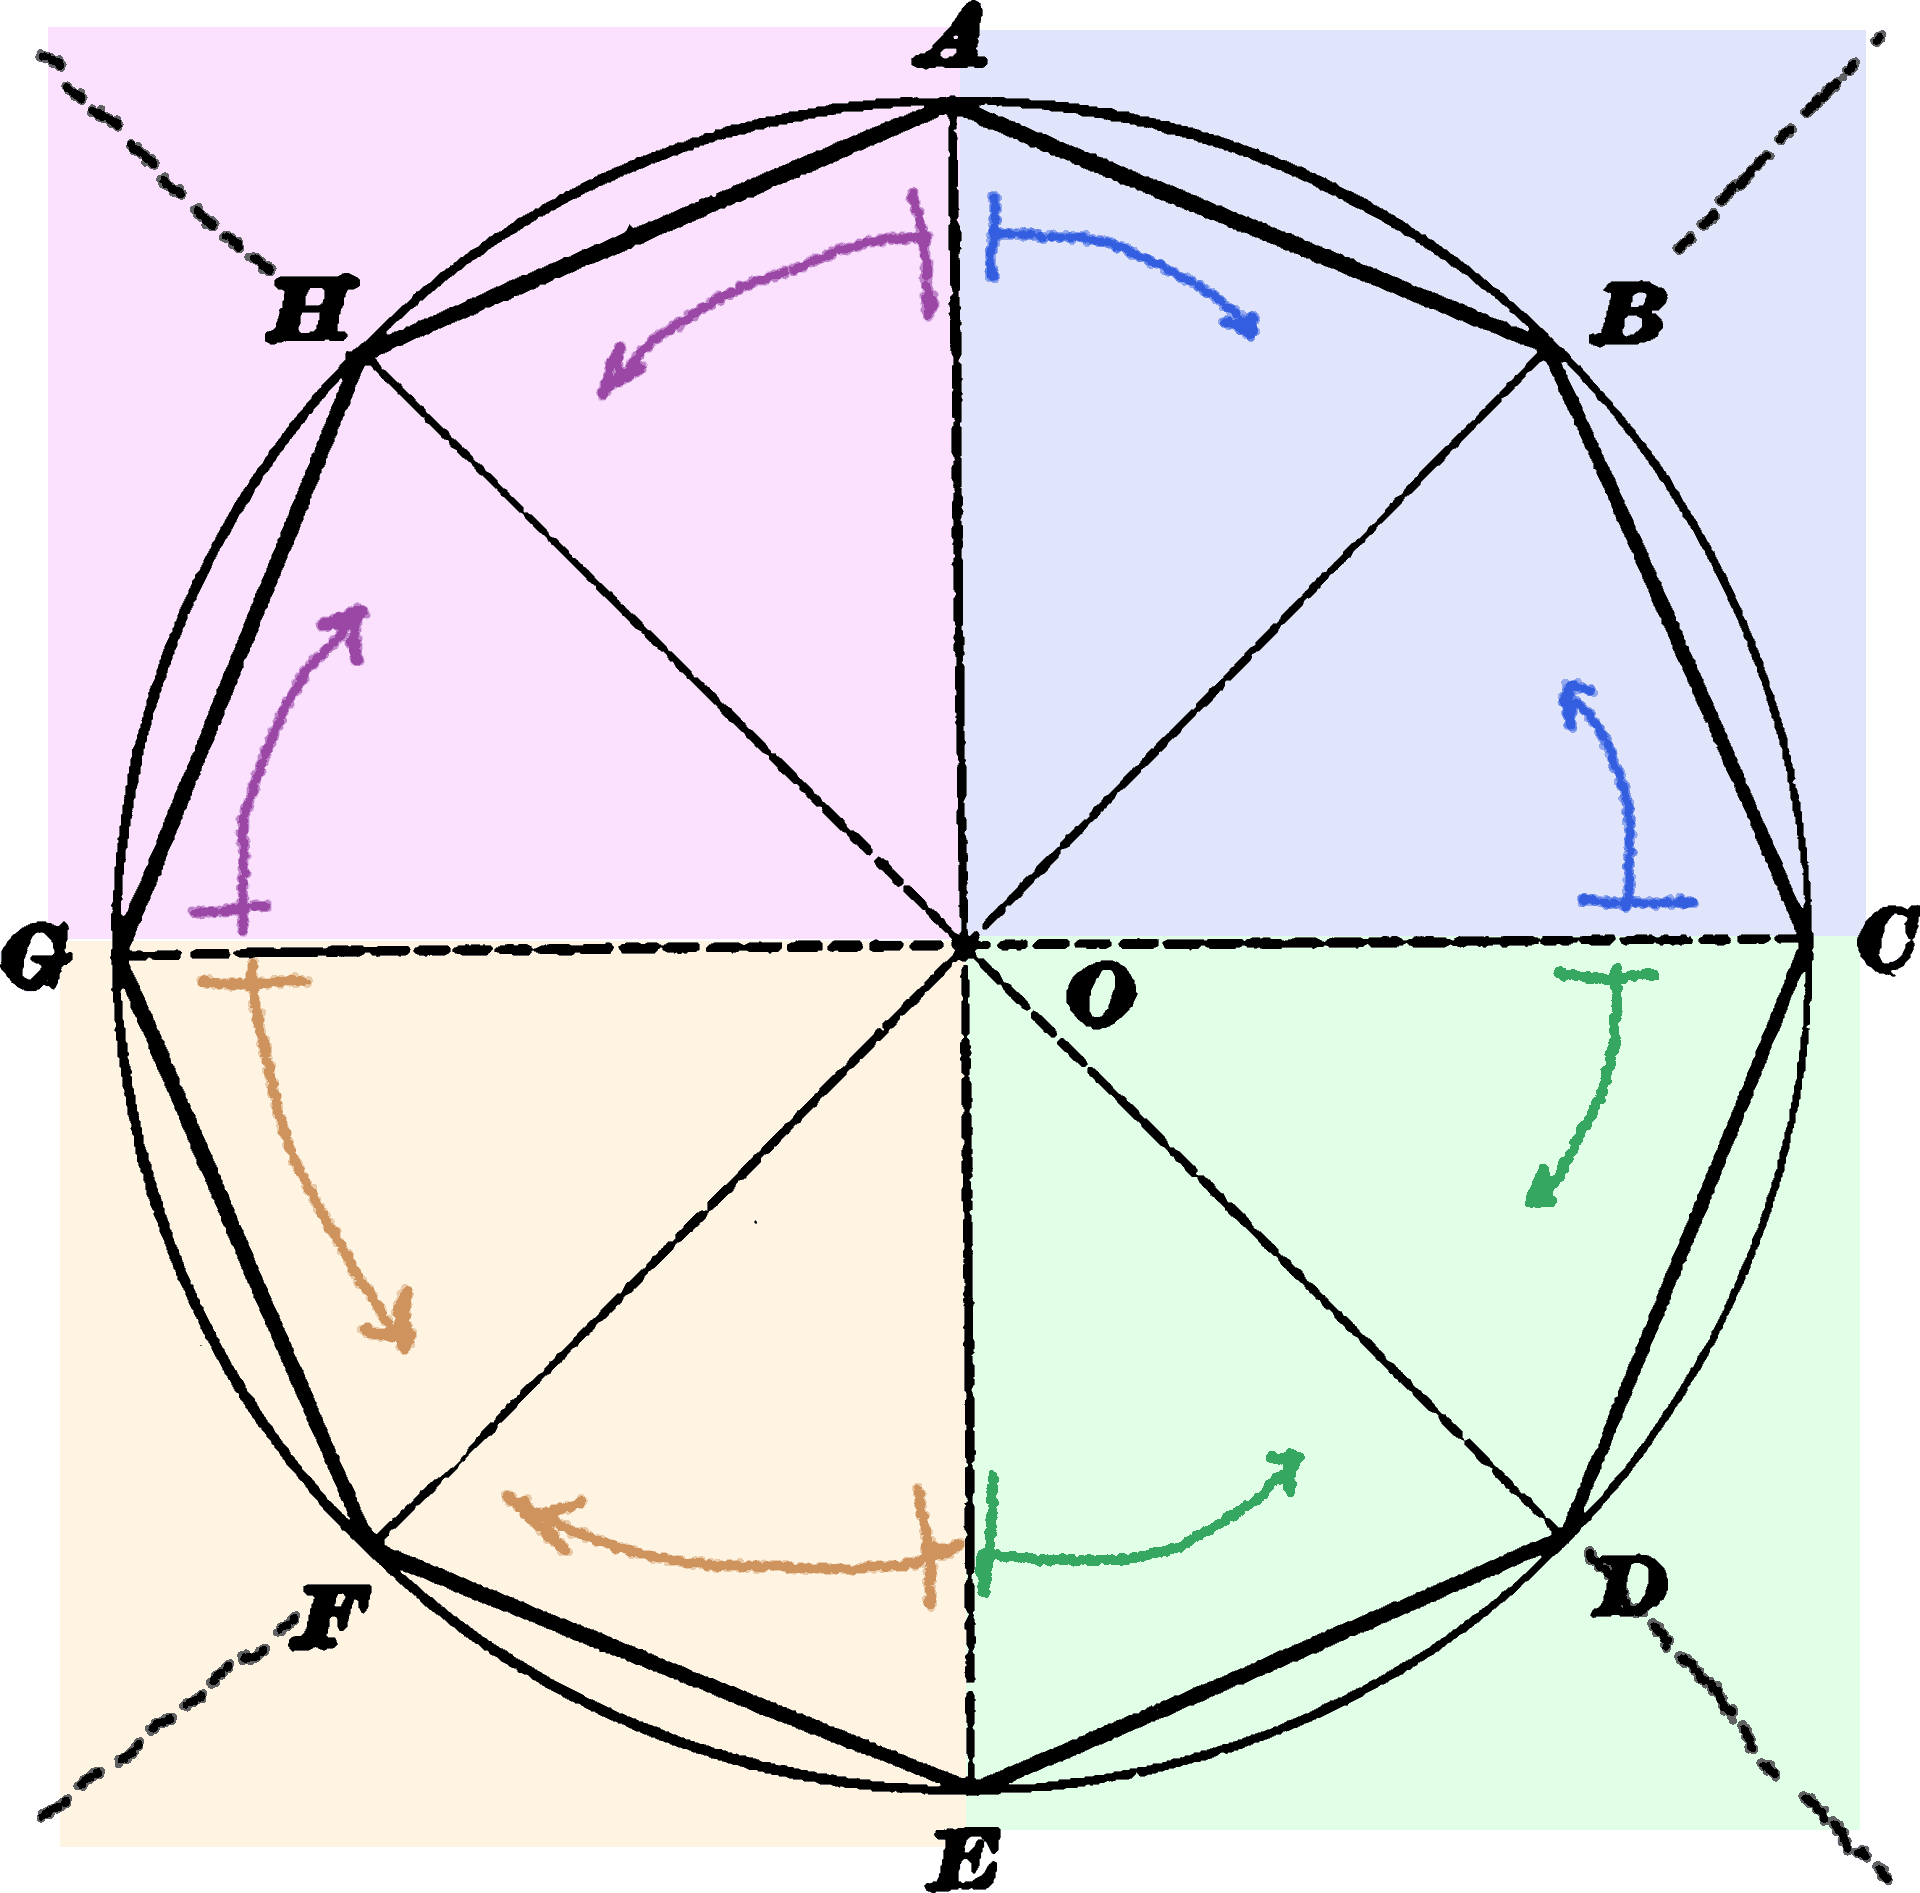
\includegraphics[width=.9\linewidth]{images/circle-8way.png}
\caption{We choose 8-way symmetry of the circle for computational efficiency.}
\end{figure}
\end{column}
\end{columns}
\end{frame}

\begin{frame}[label={sec:orga6a893f}]{efficient computation}
\begin{columns}
\begin{column}{.45\columnwidth}
\begin{figure}[htbp]
\centering
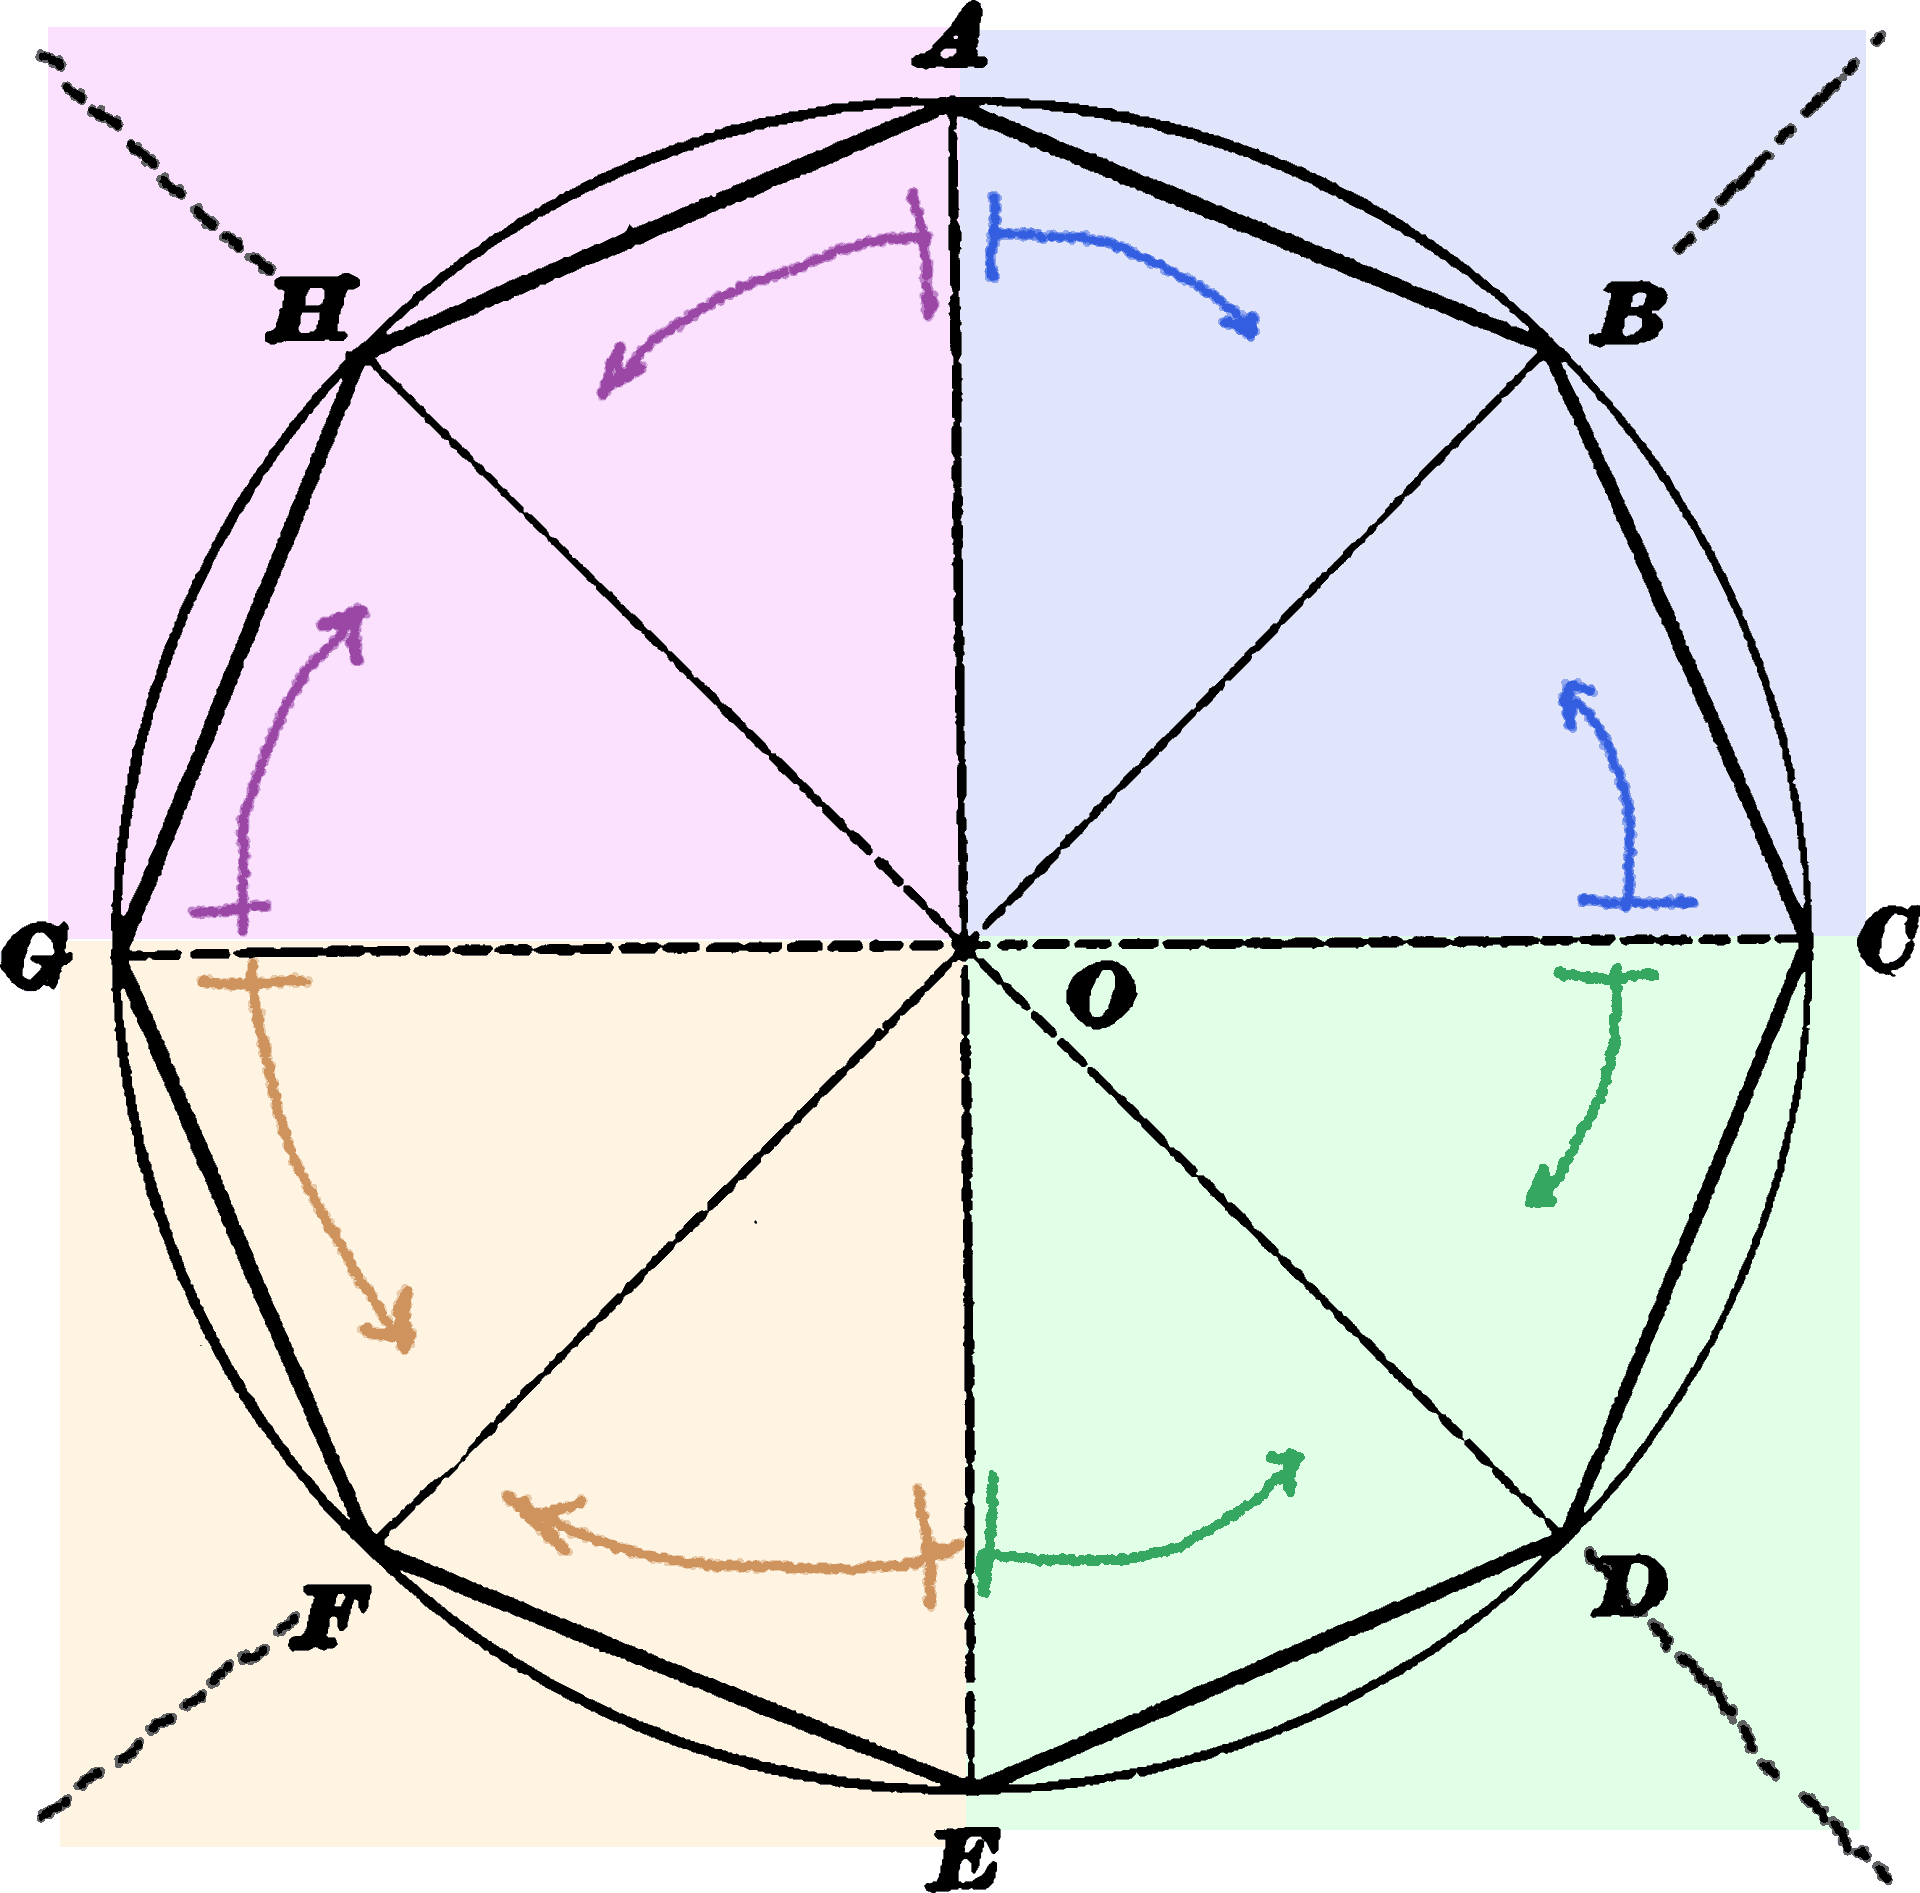
\includegraphics[width=.9\linewidth]{images/circle-8way.png}
\caption{We choose 8-way symmetry of the circle for computational efficiency.}
\end{figure}
\end{column}


\begin{column}{.55\columnwidth}
Computing the points on any one of the eight
symmetrical sectors (\alert{octant}), gives us the points on
the other seven.

Let \((x,y)\) be the point on one octant, the other seven
are given as,
\begin{enumerate}
\item \((x,-y)\)
\item \((-x,y)\)
\item \((-x,-y)\)
\item \((y,x)\)
\item \((y,-x)\)
\item \((-y,x)\)
\item \((-y,-x)\)
\end{enumerate}
\end{column}
\end{columns}
\end{frame}

\begin{frame}[label={sec:orgdaef755}]{setup}
\begin{columns}
\begin{column}{.4\columnwidth}
\begin{center}
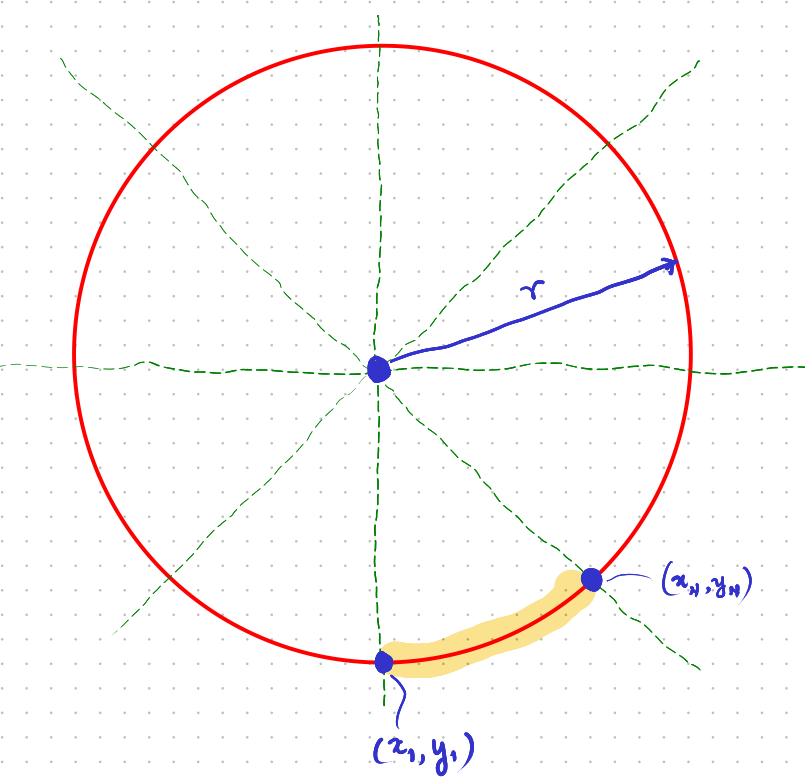
\includegraphics[width=.9\linewidth]{org-download-images/mid-point_algorithm/2024-09-03_21-50-20_screenshot.png}
\end{center}
\end{column}

\begin{column}{.6\columnwidth}
Given a circle with radius \(r\), centred at origin, we
intend to compute the points on (or nearest to) the
circle within the octant defined by end points,

\begin{align*}
  \begin{bmatrix} x_1 \\ y_1 \end{bmatrix}
  &= \begin{bmatrix} 0 \\ -r \end{bmatrix} \\
  \begin{bmatrix} x_N \\ y_N \end{bmatrix}
  &= \begin{bmatrix} \lceil\frac{r}{\sqrt{2}}\rceil \\
    -\lceil\frac{r}{\sqrt{2}}\rceil \end{bmatrix}
\end{align*}
\end{column}
\end{columns}
\end{frame}


\begin{frame}[label={sec:org1aff3dd}]{at iteration \(t\)}
\begin{columns}
\begin{column}{.4\columnwidth}
\begin{center}
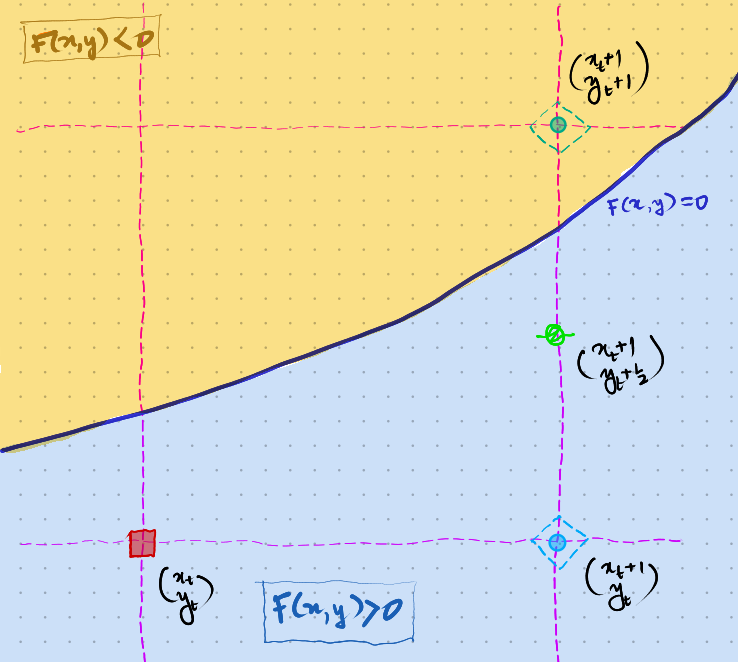
\includegraphics[width=.9\linewidth]{org-download-images/mid-point_algorithm/2024-09-03_22-08-34_screenshot.png}
\end{center}
\end{column}


\begin{column}{.6\columnwidth}
\begin{align*}
  F(x, y) &= x^2 + y^2 - r^2
\end{align*}

At timestep \(t\), let \((x_{t}, y_{t})\) be the point
closest to the curve given by \(F(x,y)=0\).
\end{column}
\end{columns}
\end{frame}
\begin{frame}[label={sec:org5391a80}]{at iteration \(t+1\)}
\begin{columns}
\begin{column}{.4\columnwidth}
\begin{center}
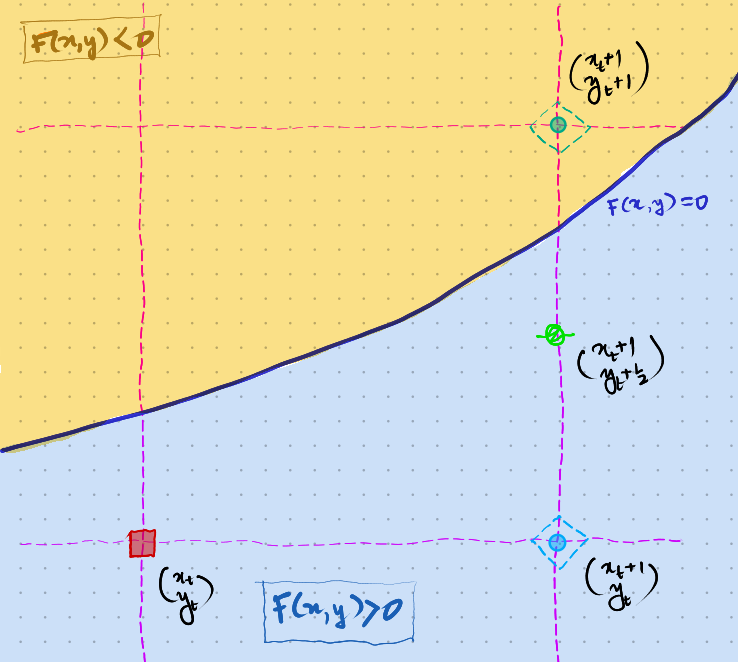
\includegraphics[width=.9\linewidth]{org-download-images/mid-point_algorithm/2024-09-03_22-08-34_screenshot.png}
\end{center}
\end{column}


\begin{column}{.6\columnwidth}
\begin{align*}
  \alert{x_{t+1}}
  &= x_{t} + 1 \\
  \alert{y_{t+1}}
  &= y_{t} + I[\delta_{t+1}>0]
    \only<2-4>{ \\
  \delta_{t+1}
  &= F(x_{t}+1,y_{t}+\frac12) \\
  &= x_t^2 + 2x_t+1+y_t^2+y_t+\frac14-r^2}
    \only<3-4>{ \\
  \delta_t
  &= F(x_{t-1}+1,y_{t-1}+\frac12) =
    F(x_{t},y_{t-1}+\frac12) \\
  &= x_t^2+y_{t-1}^2+y_{t-1}+\frac14-r^2 }
    \only<4-5>{ \\
  \delta_{t+1}-\delta_t
  &= 2x_t+1+(y_{t}-y_{t-1})(y_{t}+y_{t-1}+1) }
    \only<5-6>{ \\
  \alert{\delta_{t+1}}
  &= \delta_t + 2x_t+1 + I[\delta_t>0]\cdot(2y_t)
    }
\end{align*}
\end{column}
\end{columns}
\end{frame}

\begin{frame}[label={sec:orgf1ab005}]{boundary conditions}
\begin{columns}
\begin{column}{.3\columnwidth}
\begin{center}
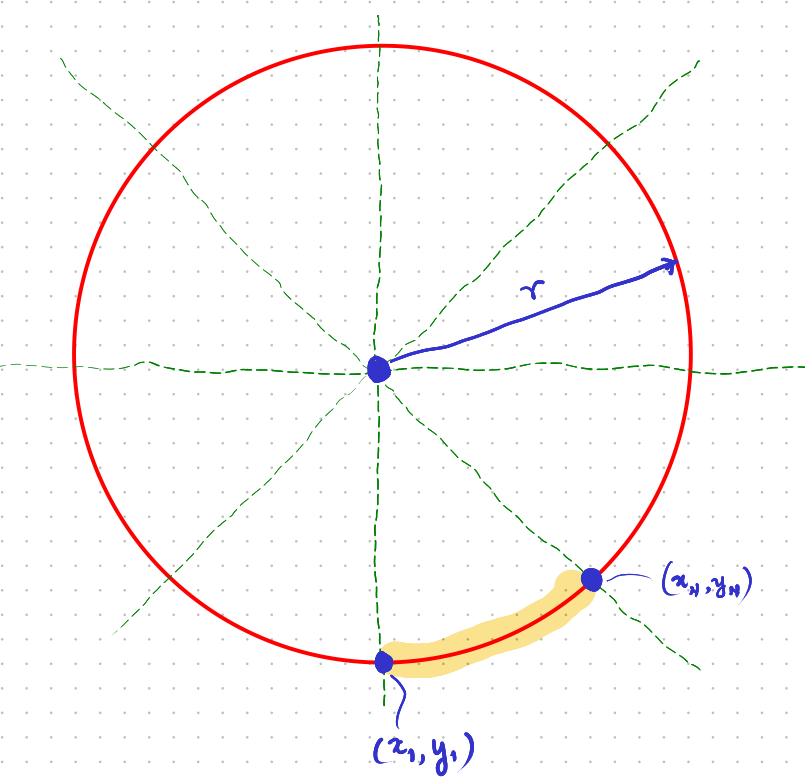
\includegraphics[width=.9\linewidth]{org-download-images/mid-point_algorithm/2024-09-03_21-50-20_screenshot.png}
\end{center}

\begin{align*}
  \begin{bmatrix} x_1 & x_N \\ y_1 & y_N \end{bmatrix}
  &= \begin{bmatrix}
    0 & \lceil\frac{r}{\sqrt{2}}\rceil \\
    -r & -\lceil\frac{r}{\sqrt{2}}\rceil \end{bmatrix}
\end{align*}
\end{column}

\begin{column}{.35\columnwidth}
\begin{center}
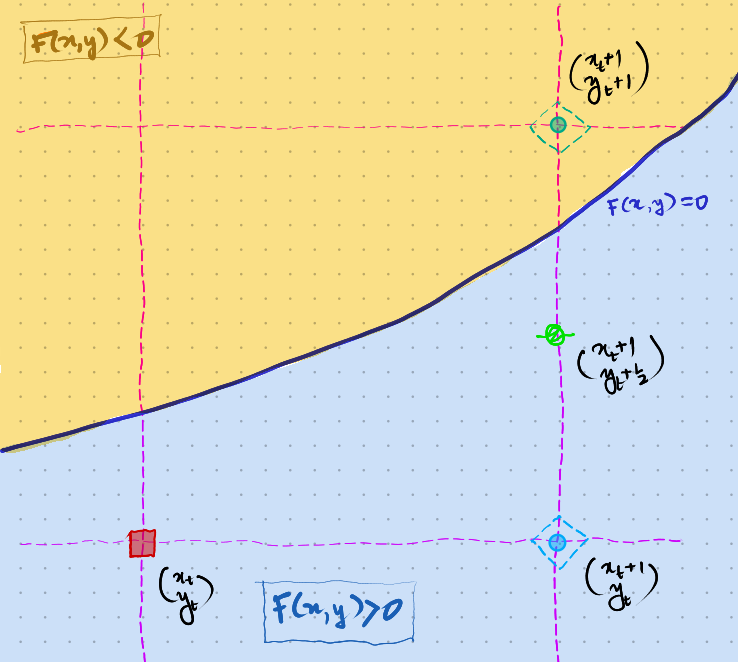
\includegraphics[width=.9\linewidth]{org-download-images/mid-point_algorithm/2024-09-03_22-08-34_screenshot.png}
\end{center}
\begin{align*}
  \delta_2 &= F(x_{2},y_{1}+\frac12) &&= F(1,-r+\frac12) \\
           &= 1-r+\frac14 &&\approx 1-r
\end{align*}
\end{column}
\end{columns}
\end{frame}


\againframe{sec:orgcb7baa7}

\begin{frame}[label={sec:org8032ea1}]{midpoint algo for circle octant}
\begin{algorithm}[H]
  \caption{Mid-Point Algorithm for Circle Octant}
  \DontPrintSemicolon

  \Fn(\hfill {\scriptsize Base case.}){\upshape
    $\textsc{mid-point-algo-octant}\, (r)$}{
    \KwIn{$r \in \mathbb{Z} \vdash 0<r$ \hfill
      \scriptsize Radius of the circle.}

    \KwOut{$C \equiv \{(x_1,y_1),\ldots,(x_N,y_N) \}
      \subset \mathbb{Z}^2$ \\\scriptsize An ordered
      sequence; a curve in discrete 2D space.}

    $C\gets\emptyset$ \hfill {\scriptsize Initialise
      array.}

    $(x,y,\delta,N) \gets (0, -r, 1-r, \lceil
    \frac{r}{\sqrt{2}} \rceil)$ \hfill {\scriptsize
      Initialise with boundary condition.}

    $C\cdot\textsc{push}((x,y))$\hfill {\scriptsize
      $(x,y)$ is a tuple.}

    \For(\hfill{\scriptsize Iterate over
      $x$}){$x\in\{1,\ldots,N\}$}{

      $y\gets y+I[\delta>0]$

      $C\cdot\textsc{push}((x,y))$\hfill {\scriptsize
        $(x,y)$ is a tuple.}

      $\delta \gets \delta + 2x + 1 +
      I[\delta>0]\cdot(2y)$

    }

    \Return $C$

  }
\end{algorithm}
\end{frame}

\begin{frame}[label={sec:orgccddf7c}]{midpoint algo for circle octant}
\begin{algorithm}[H]
  \caption{Mid-Point Algorithm for Circle}
  \DontPrintSemicolon

  \Fn(\hfill {\scriptsize All cases.}){\upshape
    $\textsc{mid-point-algo-circle}\, (r)$}{
    \KwIn{$r \in \mathbb{Z} \vdash 0<r$ \hfill
      \scriptsize Radius of the circle.}

    \KwOut{$C \equiv \{(x_1,y_1),\ldots,(x_N,y_N) \}
      \subset \mathbb{Z}^2$ \\\scriptsize An ordered
      sequence; a curve in discrete 2D space.}

    $C\gets\textsc{mid-point-algo-circle}\, (r)$ \hfill
    {\scriptsize Initialise with octant points.}

    \textbf{define:} $\textsc{quad-sym}\,((x,y))
    \mapsto [(x,y),(x,-y),(-x,y),(-x,-y)]$

    \textbf{define:}
    $\textsc{oct-sym}\,((x,y)) \mapsto
    \textsc{concat}\, (\textsc{quad-sym}\,((x,y)),
    \textsc{quad-sym}\,((y,x)))$

    $C\gets \textsc{map-concat}\,(\textsc{oct-sym}, C)$

    \Return $C$

  }
\end{algorithm}
\end{frame}

\subsection{Ellipse}
\label{sec:org076b752}

\begin{frame}[label={sec:org903343a}]{symmetry}
\begin{figure}[htbp]
\centering
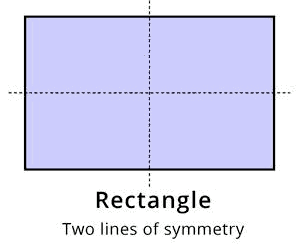
\includegraphics[width=.9\linewidth]{images/rect-symmetry.png}
\caption{Rectangular Symmetry}
\end{figure}
\end{frame}

\begin{frame}[label={sec:org9b01c26}]{computational efficiency}
\begin{center}
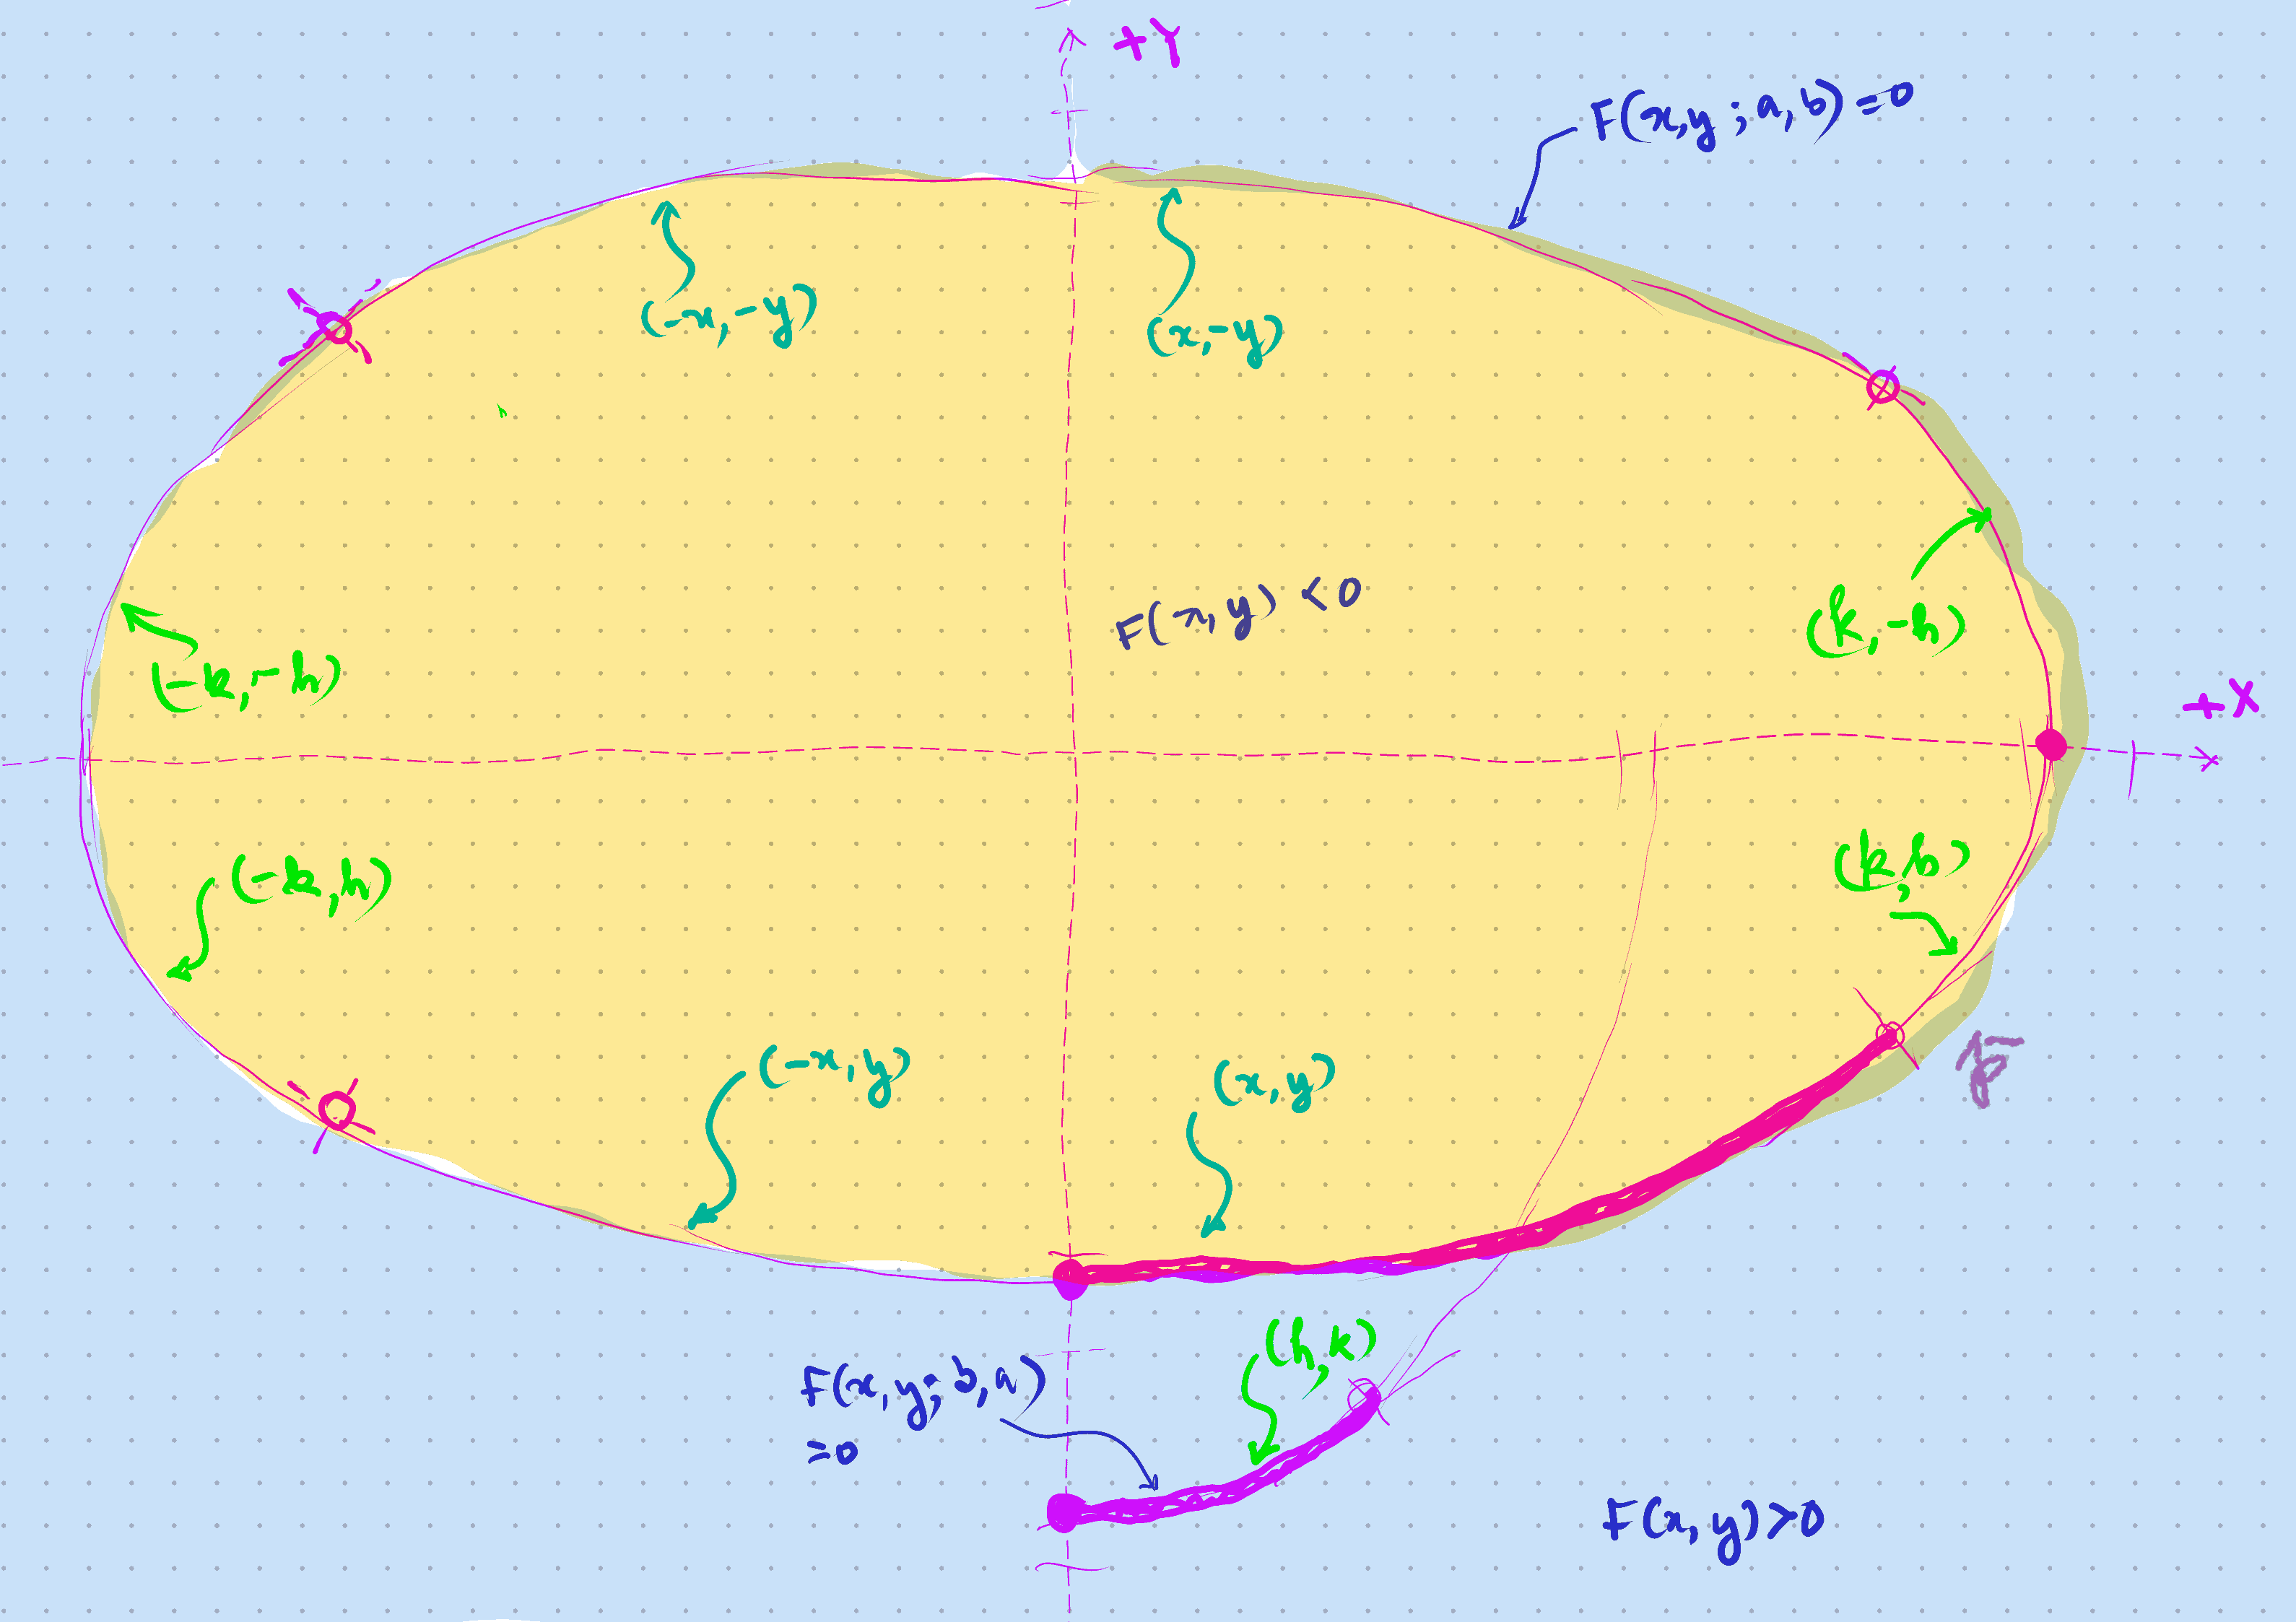
\includegraphics[width=.9\linewidth]{images/2024-09-05-Note-15-30_annotated.png}
\end{center}
\end{frame}

\begin{frame}[label={sec:org134d448}]{signed distance function (sdf) of ellipse}
\begin{align*}
  \frac{x^2}{a^2} + \frac{y^2}{b^2}
  &= 1
  \\
  F(x,y;a,b)
  &= b^2x^2+z^2y^2-a^2b^2
\end{align*}
\end{frame}

\begin{frame}[label={sec:org6dab684}]{point of inflection}
\begin{align*}
  \frac{x^2}{a^2}+\frac{y^2}{b^2}
  &= 1 \\
  \frac{2x\mathrm{d}x}{a^2} + \frac{2y\mathrm{d}y}{b^2}
  &= 0 \\
  \left.\frac{\mathrm{d}y}{\mathrm{d}x}
  \right\vert_{\mathbf{p}}
  = -\frac{b^2x_p}{a^2y_p}
  &=1 \\
  x_p
  &= -\frac{a^2y_p}{b^2} \\
  &= \pm \frac{a^2}{\sqrt{a^2+b^2}}
\end{align*}
\end{frame}

\begin{frame}[label={sec:org32d7012}]{at iteration \(t\)}
\begin{columns}
\begin{column}{.45\columnwidth}
Let point \((x_{t},y_{t})\) be closest to the theoretical
curve,
\end{column}
\end{columns}
\end{frame}

\begin{frame}[label={sec:org070c1e6}]{at iteration \(t+1\)}
\begin{align*}
  \alert{x_{t+1}}
  &= x_t+1 \\
  \alert{y_{t+1}}
  &=y_t+I[\delta_{t+1}>0]
  \only<2-5>{ \\
  \delta_{t+1}
  &=F(x_t+1,y_t+\frac12) \\
  &=b^2(x_t+1)^2+a^2(y_t+\frac12)^2-a^2b^2
    }\only<3-5>{ \\
  &=b^2x_t^2+2b^2x_t+b^2 + a^2y_t^2 + a^2y_t+a^2 -
    a^2b^2 
    }\only<4-5>{ \\
  \delta_t
  &= b^2x_t^2+ a^2y_{t-1}^2 + a^2y_{t-1}+a^2 - a^2b^2
    }\only<5-6>{ \\
  \delta_{t+1}-\delta_t
  &= 2b^2x_t+b^2+a^2(y_{t+1}-y_t)(y_{t+1}+y_t+1)
    } \only<6>{ \\
  \alert{\delta_{t+1}}
  &= \delta_t + 2b^2x_t+b^2+I[\delta_t>0]\cdot(2a^2y_t)
    }
\end{align*}
\end{frame}

\begin{frame}[label={sec:org0f8dc4d}]{boundary conditions}
at t=1, \(x=0, y=-b\)

at t=2,
\begin{align*}
  \delta_{2}
  &=F(x_{1}+1,y_{1}+\frac12) \\
  &=b^2 + a^2(-b+\frac12)^2-a^2b^2 \\
  &=b^2-a^2b+\frac{a^2}{4}
\end{align*}
\end{frame}


\begin{frame}[label={sec:orgd3fcb15}]{putting it all together}
\begin{align*}
  x_1&=0 \\
  y_1&=-b \\
  \delta_{2}&=b^2-a^2b+\frac{a^2}{4} \\
  N &= \frac{a^2}{\sqrt{a^2+b^2}} \\
  x_{t+1} &= x_t+1 \\
  y_{t+1} &= y_t+I[\delta_{t+1}>0] \\
  \delta_{t+1} &= \delta_t + 2b^2x_t+b^2 +
                 I[\delta_t>0]\cdot(2a^2y_t)
\end{align*}
\end{frame}

\begin{frame}[label={sec:org5d4716c}]{midpoint algorithm for ellipse}
\begin{algorithm}[H]
  \caption{Mid Point Algorithm for Ellispe (BottomRight)}
  \DontPrintSemicolon

  \Fn(\hfill {\scriptsize Base Case.}){\upshape
    $\textsc{mid-point-algo-ellipse-br}\, (a,b)$}{
    \KwIn{$a,b \in \mathbb{Z} \vdash 0<a,b$ \hfill
      \scriptsize Semi-axes-lengths of the ellipse.}

    \KwOut{$C \equiv \{(x_1,y_1),\ldots,(x_N,y_N) \}
      \subset \mathbb{Z}^2$ \\\scriptsize An ordered
      sequence; a curve in discrete 2D space.}

    $C\gets\emptyset$

    $(x,y,\delta)\gets(0,-b,b^2-a^2b +
    \lceil\frac{a^2}{4}\rceil)$

    $C\cdot\textsc{push}((x,y))$

    $N\gets \lceil\frac{a^2}{\sqrt{a^2+b^2}}\rceil$

    \For(\hfill{\scriptsize Iterate along the x-axis.})
    {$x\in\{1,\ldots,N\}$} {

      $y\gets y+I[\delta>0]$
      
      $C\cdot\textsc{push}((x,y))$

      $\delta\gets \delta + 2b^2x+b^2 +
      I[\delta>0]\cdot(2a^2y)$

    }

    \Return $C$.

  }    
\end{algorithm}
\end{frame}

\begin{frame}[label={sec:org7152516}]{midpoint algorithm for ellipse}
\begin{algorithm}[H]
  \caption{Mid Point Algorithm for Ellispe (Collect
    Symmetric Points)}
  \DontPrintSemicolon

  \Fn(\hfill {\scriptsize All cases.}){\upshape
    $\textsc{mid-point-algo-ellipse}\, (a,b)$}{
    \KwIn{$a,b \in \mathbb{Z} \vdash 0<a,b$ \hfill
      \scriptsize Semi-axes-lengths of the ellipse.}

    \KwOut{$C \equiv \{(x_1,y_1),\ldots,(x_N,y_N) \}
      \subset \mathbb{Z}^2$ \\\scriptsize An ordered
      sequence; a curve in discrete 2D space.}

    $C_1\gets\textsc{mid-point-algo-ellipse-br}\, (a,b)$
    \hfill {\scriptsize Collect Bottom Right For (a,b)}

    \textbf{define:}  $\textsc{quad-sym}:((x,y))
    \mapsto [(x,y), (x,-y), (-x,y), (-x,-y)]$

    $C_1\gets\textsc{map-concat}(\textsc{quad-sym},C_1)$
    \hfill {\scriptsize Collect \textsc{quad-sym} for
      $C_1$.}

    $C_2\gets\textsc{mid-point-algo-ellipse-br}\, (b,a)$
    \hfill {\scriptsize Collect Bottom Right For (b,a)}

    \textbf{define:}  $\textsc{quad-sym-flip}:((x,y))
    \mapsto \textsc{quad-sym}((y,x))$

    $C_2\gets\textsc{map-concat}(\textsc{quad-sym-flip},C_2)$
    \hfill {\scriptsize Collect flipped
      \textsc{quad-sym} for $C_2$.}

    $C\gets\textsc{concat}(C_1, C_2)$

    \Return $C$.

  }    
\end{algorithm}
\end{frame}
\end{document}
